\documentclass[conference]{IEEEtran}
\IEEEoverridecommandlockouts
\usepackage{iftex}
\ifTUTeX % tectonic / XeLaTeX: Times clone as required by IEEEtran
  \usepackage{fontspec}
  \setmainfont{texgyretermes-regular.otf}[BoldFont=texgyretermes-bold.otf,
    ItalicFont=texgyretermes-italic.otf, BoldItalicFont=texgyretermes-bolditalic.otf]
\else
  \usepackage[T1]{fontenc}
  \usepackage[utf8]{inputenc}
\fi
\usepackage{cite}
\usepackage{amsmath,amssymb}
\usepackage{graphicx}
\usepackage{booktabs}
\usepackage{xcolor}
\usepackage{tikz}
\usetikzlibrary{positioning,arrows.meta,fit}
\usepackage[hidelinks]{hyperref}
\usepackage{url}
% AUTO-GENERATED by scripts/95_make_paper_numbers.py - do not edit
\newcommand{\FoneBamcdOneManavgat}{0.921}
\newcommand{\FoneStdBamcdOneManavgat}{0.000}
\newcommand{\IoUBamcdOneManavgat}{0.854}
\newcommand{\IoUStdBamcdOneManavgat}{0.000}
\newcommand{\PrecBamcdOneManavgat}{0.953}
\newcommand{\PrecStdBamcdOneManavgat}{0.000}
\newcommand{\RecBamcdOneManavgat}{0.892}
\newcommand{\RecStdBamcdOneManavgat}{0.000}
\newcommand{\OABamcdOneManavgat}{0.950}
\newcommand{\OAStdBamcdOneManavgat}{0.000}
\newcommand{\AreaBamcdOneManavgat}{50\,922}
\newcommand{\RefAreaManavgat}{54\,367}
\newcommand{\FoneBamcdTwoManavgat}{0.931}
\newcommand{\FoneStdBamcdTwoManavgat}{0.000}
\newcommand{\IoUBamcdTwoManavgat}{0.872}
\newcommand{\IoUStdBamcdTwoManavgat}{0.000}
\newcommand{\PrecBamcdTwoManavgat}{0.939}
\newcommand{\PrecStdBamcdTwoManavgat}{0.000}
\newcommand{\RecBamcdTwoManavgat}{0.924}
\newcommand{\RecStdBamcdTwoManavgat}{0.000}
\newcommand{\OABamcdTwoManavgat}{0.955}
\newcommand{\OAStdBamcdTwoManavgat}{0.000}
\newcommand{\AreaBamcdTwoManavgat}{53\,479}
\newcommand{\RefAreaManavgat}{54\,367}
\newcommand{\FoneDnbrFlogaManavgat}{0.822}
\newcommand{\FoneStdDnbrFlogaManavgat}{0.000}
\newcommand{\IoUDnbrFlogaManavgat}{0.698}
\newcommand{\IoUStdDnbrFlogaManavgat}{0.000}
\newcommand{\PrecDnbrFlogaManavgat}{0.949}
\newcommand{\PrecStdDnbrFlogaManavgat}{0.000}
\newcommand{\RecDnbrFlogaManavgat}{0.725}
\newcommand{\RecStdDnbrFlogaManavgat}{0.000}
\newcommand{\OADnbrFlogaManavgat}{0.896}
\newcommand{\OAStdDnbrFlogaManavgat}{0.000}
\newcommand{\AreaDnbrFlogaManavgat}{41\,524}
\newcommand{\RefAreaManavgat}{54\,367}
\newcommand{\FoneDnbrLowManavgat}{0.882}
\newcommand{\FoneStdDnbrLowManavgat}{0.000}
\newcommand{\IoUDnbrLowManavgat}{0.789}
\newcommand{\IoUStdDnbrLowManavgat}{0.000}
\newcommand{\PrecDnbrLowManavgat}{0.886}
\newcommand{\PrecStdDnbrLowManavgat}{0.000}
\newcommand{\RecDnbrLowManavgat}{0.878}
\newcommand{\RecStdDnbrLowManavgat}{0.000}
\newcommand{\OADnbrLowManavgat}{0.922}
\newcommand{\OAStdDnbrLowManavgat}{0.000}
\newcommand{\AreaDnbrLowManavgat}{53\,919}
\newcommand{\RefAreaManavgat}{54\,367}
\newcommand{\FoneDnbrModManavgat}{0.797}
\newcommand{\FoneStdDnbrModManavgat}{0.000}
\newcommand{\IoUDnbrModManavgat}{0.663}
\newcommand{\IoUStdDnbrModManavgat}{0.000}
\newcommand{\PrecDnbrModManavgat}{0.956}
\newcommand{\PrecStdDnbrModManavgat}{0.000}
\newcommand{\RecDnbrModManavgat}{0.684}
\newcommand{\RecStdDnbrModManavgat}{0.000}
\newcommand{\OADnbrModManavgat}{0.885}
\newcommand{\OAStdDnbrModManavgat}{0.000}
\newcommand{\AreaDnbrModManavgat}{38\,887}
\newcommand{\RefAreaManavgat}{54\,367}
\newcommand{\FoneLgbmManavgat}{0.882}
\newcommand{\FoneStdLgbmManavgat}{0.001}
\newcommand{\IoULgbmManavgat}{0.789}
\newcommand{\IoUStdLgbmManavgat}{0.001}
\newcommand{\PrecLgbmManavgat}{0.931}
\newcommand{\PrecStdLgbmManavgat}{0.001}
\newcommand{\RecLgbmManavgat}{0.838}
\newcommand{\RecStdLgbmManavgat}{0.002}
\newcommand{\OALgbmManavgat}{0.926}
\newcommand{\OAStdLgbmManavgat}{0.000}
\newcommand{\AreaLgbmManavgat}{48\,943}
\newcommand{\RefAreaManavgat}{54\,367}
\newcommand{\FoneAblGOneManavgat}{0.819}
\newcommand{\FoneStdAblGOneManavgat}{0.004}
\newcommand{\IoUAblGOneManavgat}{0.693}
\newcommand{\IoUStdAblGOneManavgat}{0.006}
\newcommand{\PrecAblGOneManavgat}{0.950}
\newcommand{\PrecStdAblGOneManavgat}{0.001}
\newcommand{\RecAblGOneManavgat}{0.720}
\newcommand{\RecStdAblGOneManavgat}{0.007}
\newcommand{\OAAblGOneManavgat}{0.895}
\newcommand{\OAStdAblGOneManavgat}{0.002}
\newcommand{\AreaAblGOneManavgat}{41\,172}
\newcommand{\RefAreaManavgat}{54\,367}
\newcommand{\FoneAblGTwoManavgat}{0.862}
\newcommand{\FoneStdAblGTwoManavgat}{0.001}
\newcommand{\IoUAblGTwoManavgat}{0.758}
\newcommand{\IoUStdAblGTwoManavgat}{0.002}
\newcommand{\PrecAblGTwoManavgat}{0.936}
\newcommand{\PrecStdAblGTwoManavgat}{0.001}
\newcommand{\RecAblGTwoManavgat}{0.799}
\newcommand{\RecStdAblGTwoManavgat}{0.003}
\newcommand{\OAAblGTwoManavgat}{0.916}
\newcommand{\OAStdAblGTwoManavgat}{0.001}
\newcommand{\AreaAblGTwoManavgat}{46\,397}
\newcommand{\RefAreaManavgat}{54\,367}
\newcommand{\FoneAblGTwoThreeManavgat}{0.874}
\newcommand{\FoneStdAblGTwoThreeManavgat}{0.001}
\newcommand{\IoUAblGTwoThreeManavgat}{0.777}
\newcommand{\IoUStdAblGTwoThreeManavgat}{0.001}
\newcommand{\PrecAblGTwoThreeManavgat}{0.936}
\newcommand{\PrecStdAblGTwoThreeManavgat}{0.001}
\newcommand{\RecAblGTwoThreeManavgat}{0.820}
\newcommand{\RecStdAblGTwoThreeManavgat}{0.002}
\newcommand{\OAAblGTwoThreeManavgat}{0.922}
\newcommand{\OAStdAblGTwoThreeManavgat}{0.000}
\newcommand{\AreaAblGTwoThreeManavgat}{47\,647}
\newcommand{\RefAreaManavgat}{54\,367}
\newcommand{\FoneLogregManavgat}{0.832}
\newcommand{\FoneStdLogregManavgat}{0.000}
\newcommand{\IoULogregManavgat}{0.713}
\newcommand{\IoUStdLogregManavgat}{0.000}
\newcommand{\PrecLogregManavgat}{0.939}
\newcommand{\PrecStdLogregManavgat}{0.000}
\newcommand{\RecLogregManavgat}{0.748}
\newcommand{\RecStdLogregManavgat}{0.000}
\newcommand{\OALogregManavgat}{0.901}
\newcommand{\OAStdLogregManavgat}{0.000}
\newcommand{\AreaLogregManavgat}{43\,304}
\newcommand{\RefAreaManavgat}{54\,367}
\newcommand{\FoneRfManavgat}{0.886}
\newcommand{\FoneStdRfManavgat}{0.000}
\newcommand{\IoURfManavgat}{0.795}
\newcommand{\IoUStdRfManavgat}{0.001}
\newcommand{\PrecRfManavgat}{0.928}
\newcommand{\PrecStdRfManavgat}{0.000}
\newcommand{\RecRfManavgat}{0.848}
\newcommand{\RecStdRfManavgat}{0.001}
\newcommand{\OARfManavgat}{0.928}
\newcommand{\OAStdRfManavgat}{0.000}
\newcommand{\AreaRfManavgat}{49\,669}
\newcommand{\RefAreaManavgat}{54\,367}
\newcommand{\FoneBamcdOneMarmaris}{0.866}
\newcommand{\FoneStdBamcdOneMarmaris}{0.000}
\newcommand{\IoUBamcdOneMarmaris}{0.764}
\newcommand{\IoUStdBamcdOneMarmaris}{0.000}
\newcommand{\PrecBamcdOneMarmaris}{0.984}
\newcommand{\PrecStdBamcdOneMarmaris}{0.000}
\newcommand{\RecBamcdOneMarmaris}{0.774}
\newcommand{\RecStdBamcdOneMarmaris}{0.000}
\newcommand{\OABamcdOneMarmaris}{0.919}
\newcommand{\OAStdBamcdOneMarmaris}{0.000}
\newcommand{\AreaBamcdOneMarmaris}{9\,073}
\newcommand{\RefAreaMarmaris}{11\,541}
\newcommand{\FoneBamcdTwoMarmaris}{0.893}
\newcommand{\FoneStdBamcdTwoMarmaris}{0.000}
\newcommand{\IoUBamcdTwoMarmaris}{0.806}
\newcommand{\IoUStdBamcdTwoMarmaris}{0.000}
\newcommand{\PrecBamcdTwoMarmaris}{0.979}
\newcommand{\PrecStdBamcdTwoMarmaris}{0.000}
\newcommand{\RecBamcdTwoMarmaris}{0.821}
\newcommand{\RecStdBamcdTwoMarmaris}{0.000}
\newcommand{\OABamcdTwoMarmaris}{0.933}
\newcommand{\OAStdBamcdTwoMarmaris}{0.000}
\newcommand{\AreaBamcdTwoMarmaris}{9\,670}
\newcommand{\RefAreaMarmaris}{11\,541}
\newcommand{\FoneDnbrFlogaMarmaris}{0.831}
\newcommand{\FoneStdDnbrFlogaMarmaris}{0.000}
\newcommand{\IoUDnbrFlogaMarmaris}{0.711}
\newcommand{\IoUStdDnbrFlogaMarmaris}{0.000}
\newcommand{\PrecDnbrFlogaMarmaris}{0.980}
\newcommand{\PrecStdDnbrFlogaMarmaris}{0.000}
\newcommand{\RecDnbrFlogaMarmaris}{0.721}
\newcommand{\RecStdDnbrFlogaMarmaris}{0.000}
\newcommand{\OADnbrFlogaMarmaris}{0.900}
\newcommand{\OAStdDnbrFlogaMarmaris}{0.000}
\newcommand{\AreaDnbrFlogaMarmaris}{8\,496}
\newcommand{\RefAreaMarmaris}{11\,541}
\newcommand{\FoneDnbrLowMarmaris}{0.925}
\newcommand{\FoneStdDnbrLowMarmaris}{0.000}
\newcommand{\IoUDnbrLowMarmaris}{0.860}
\newcommand{\IoUStdDnbrLowMarmaris}{0.000}
\newcommand{\PrecDnbrLowMarmaris}{0.954}
\newcommand{\PrecStdDnbrLowMarmaris}{0.000}
\newcommand{\RecDnbrLowMarmaris}{0.897}
\newcommand{\RecStdDnbrLowMarmaris}{0.000}
\newcommand{\OADnbrLowMarmaris}{0.950}
\newcommand{\OAStdDnbrLowMarmaris}{0.000}
\newcommand{\AreaDnbrLowMarmaris}{10\,841}
\newcommand{\RefAreaMarmaris}{11\,541}
\newcommand{\FoneDnbrModMarmaris}{0.800}
\newcommand{\FoneStdDnbrModMarmaris}{0.000}
\newcommand{\IoUDnbrModMarmaris}{0.667}
\newcommand{\IoUStdDnbrModMarmaris}{0.000}
\newcommand{\PrecDnbrModMarmaris}{0.983}
\newcommand{\PrecStdDnbrModMarmaris}{0.000}
\newcommand{\RecDnbrModMarmaris}{0.675}
\newcommand{\RecStdDnbrModMarmaris}{0.000}
\newcommand{\OADnbrModMarmaris}{0.885}
\newcommand{\OAStdDnbrModMarmaris}{0.000}
\newcommand{\AreaDnbrModMarmaris}{7\,930}
\newcommand{\RefAreaMarmaris}{11\,541}
\newcommand{\FoneLgbmMarmaris}{0.855}
\newcommand{\FoneStdLgbmMarmaris}{0.003}
\newcommand{\IoULgbmMarmaris}{0.747}
\newcommand{\IoUStdLgbmMarmaris}{0.005}
\newcommand{\PrecLgbmMarmaris}{0.976}
\newcommand{\PrecStdLgbmMarmaris}{0.000}
\newcommand{\RecLgbmMarmaris}{0.761}
\newcommand{\RecStdLgbmMarmaris}{0.006}
\newcommand{\OALgbmMarmaris}{0.912}
\newcommand{\OAStdLgbmMarmaris}{0.002}
\newcommand{\AreaLgbmMarmaris}{9\,001}
\newcommand{\RefAreaMarmaris}{11\,541}
\newcommand{\FoneAblGOneMarmaris}{0.827}
\newcommand{\FoneStdAblGOneMarmaris}{0.005}
\newcommand{\IoUAblGOneMarmaris}{0.705}
\newcommand{\IoUStdAblGOneMarmaris}{0.007}
\newcommand{\PrecAblGOneMarmaris}{0.980}
\newcommand{\PrecStdAblGOneMarmaris}{0.001}
\newcommand{\RecAblGOneMarmaris}{0.715}
\newcommand{\RecStdAblGOneMarmaris}{0.008}
\newcommand{\OAAblGOneMarmaris}{0.898}
\newcommand{\OAStdAblGOneMarmaris}{0.003}
\newcommand{\AreaAblGOneMarmaris}{8\,421}
\newcommand{\RefAreaMarmaris}{11\,541}
\newcommand{\FoneAblGTwoMarmaris}{0.831}
\newcommand{\FoneStdAblGTwoMarmaris}{0.003}
\newcommand{\IoUAblGTwoMarmaris}{0.712}
\newcommand{\IoUStdAblGTwoMarmaris}{0.004}
\newcommand{\PrecAblGTwoMarmaris}{0.978}
\newcommand{\PrecStdAblGTwoMarmaris}{0.000}
\newcommand{\RecAblGTwoMarmaris}{0.723}
\newcommand{\RecStdAblGTwoMarmaris}{0.004}
\newcommand{\OAAblGTwoMarmaris}{0.900}
\newcommand{\OAStdAblGTwoMarmaris}{0.001}
\newcommand{\AreaAblGTwoMarmaris}{8\,530}
\newcommand{\RefAreaMarmaris}{11\,541}
\newcommand{\FoneAblGTwoThreeMarmaris}{0.875}
\newcommand{\FoneStdAblGTwoThreeMarmaris}{0.002}
\newcommand{\IoUAblGTwoThreeMarmaris}{0.778}
\newcommand{\IoUStdAblGTwoThreeMarmaris}{0.003}
\newcommand{\PrecAblGTwoThreeMarmaris}{0.976}
\newcommand{\PrecStdAblGTwoThreeMarmaris}{0.000}
\newcommand{\RecAblGTwoThreeMarmaris}{0.793}
\newcommand{\RecStdAblGTwoThreeMarmaris}{0.003}
\newcommand{\OAAblGTwoThreeMarmaris}{0.923}
\newcommand{\OAStdAblGTwoThreeMarmaris}{0.001}
\newcommand{\AreaAblGTwoThreeMarmaris}{9\,381}
\newcommand{\RefAreaMarmaris}{11\,541}
\newcommand{\FoneLogregMarmaris}{0.799}
\newcommand{\FoneStdLogregMarmaris}{0.000}
\newcommand{\IoULogregMarmaris}{0.665}
\newcommand{\IoUStdLogregMarmaris}{0.000}
\newcommand{\PrecLogregMarmaris}{0.980}
\newcommand{\PrecStdLogregMarmaris}{0.000}
\newcommand{\RecLogregMarmaris}{0.674}
\newcommand{\RecStdLogregMarmaris}{0.000}
\newcommand{\OALogregMarmaris}{0.885}
\newcommand{\OAStdLogregMarmaris}{0.000}
\newcommand{\AreaLogregMarmaris}{7\,935}
\newcommand{\RefAreaMarmaris}{11\,541}
\newcommand{\FoneRfMarmaris}{0.857}
\newcommand{\FoneStdRfMarmaris}{0.002}
\newcommand{\IoURfMarmaris}{0.750}
\newcommand{\IoUStdRfMarmaris}{0.003}
\newcommand{\PrecRfMarmaris}{0.970}
\newcommand{\PrecStdRfMarmaris}{0.001}
\newcommand{\RecRfMarmaris}{0.768}
\newcommand{\RecStdRfMarmaris}{0.004}
\newcommand{\OARfMarmaris}{0.913}
\newcommand{\OAStdRfMarmaris}{0.001}
\newcommand{\AreaRfMarmaris}{9\,136}
\newcommand{\RefAreaMarmaris}{11\,541}
\newcommand{\FoneBamcdOnePooled}{0.912}
\newcommand{\FoneStdBamcdOnePooled}{0.000}
\newcommand{\IoUBamcdOnePooled}{0.839}
\newcommand{\IoUStdBamcdOnePooled}{0.000}
\newcommand{\PrecBamcdOnePooled}{0.957}
\newcommand{\PrecStdBamcdOnePooled}{0.000}
\newcommand{\RecBamcdOnePooled}{0.872}
\newcommand{\RecStdBamcdOnePooled}{0.000}
\newcommand{\OABamcdOnePooled}{0.945}
\newcommand{\OAStdBamcdOnePooled}{0.000}
\newcommand{\AreaBamcdOnePooled}{59\,995}
\newcommand{\RefAreaPooled}{65\,908}
\newcommand{\FoneBamcdTwoPooled}{0.925}
\newcommand{\FoneStdBamcdTwoPooled}{0.000}
\newcommand{\IoUBamcdTwoPooled}{0.861}
\newcommand{\IoUStdBamcdTwoPooled}{0.000}
\newcommand{\PrecBamcdTwoPooled}{0.945}
\newcommand{\PrecStdBamcdTwoPooled}{0.000}
\newcommand{\RecBamcdTwoPooled}{0.906}
\newcommand{\RecStdBamcdTwoPooled}{0.000}
\newcommand{\OABamcdTwoPooled}{0.951}
\newcommand{\OAStdBamcdTwoPooled}{0.000}
\newcommand{\AreaBamcdTwoPooled}{63\,150}
\newcommand{\RefAreaPooled}{65\,908}
\newcommand{\FoneDnbrFlogaPooled}{0.824}
\newcommand{\FoneStdDnbrFlogaPooled}{0.000}
\newcommand{\IoUDnbrFlogaPooled}{0.700}
\newcommand{\IoUStdDnbrFlogaPooled}{0.000}
\newcommand{\PrecDnbrFlogaPooled}{0.954}
\newcommand{\PrecStdDnbrFlogaPooled}{0.000}
\newcommand{\RecDnbrFlogaPooled}{0.724}
\newcommand{\RecStdDnbrFlogaPooled}{0.000}
\newcommand{\OADnbrFlogaPooled}{0.897}
\newcommand{\OAStdDnbrFlogaPooled}{0.000}
\newcommand{\AreaDnbrFlogaPooled}{50\,020}
\newcommand{\RefAreaPooled}{65\,908}
\newcommand{\FoneDnbrLowPooled}{0.889}
\newcommand{\FoneStdDnbrLowPooled}{0.000}
\newcommand{\IoUDnbrLowPooled}{0.801}
\newcommand{\IoUStdDnbrLowPooled}{0.000}
\newcommand{\PrecDnbrLowPooled}{0.897}
\newcommand{\PrecStdDnbrLowPooled}{0.000}
\newcommand{\RecDnbrLowPooled}{0.882}
\newcommand{\RecStdDnbrLowPooled}{0.000}
\newcommand{\OADnbrLowPooled}{0.927}
\newcommand{\OAStdDnbrLowPooled}{0.000}
\newcommand{\AreaDnbrLowPooled}{64\,760}
\newcommand{\RefAreaPooled}{65\,908}
\newcommand{\FoneDnbrModPooled}{0.798}
\newcommand{\FoneStdDnbrModPooled}{0.000}
\newcommand{\IoUDnbrModPooled}{0.664}
\newcommand{\IoUStdDnbrModPooled}{0.000}
\newcommand{\PrecDnbrModPooled}{0.960}
\newcommand{\PrecStdDnbrModPooled}{0.000}
\newcommand{\RecDnbrModPooled}{0.682}
\newcommand{\RecStdDnbrModPooled}{0.000}
\newcommand{\OADnbrModPooled}{0.885}
\newcommand{\OAStdDnbrModPooled}{0.000}
\newcommand{\AreaDnbrModPooled}{46\,817}
\newcommand{\RefAreaPooled}{65\,908}
\newcommand{\FoneLgbmPooled}{0.878}
\newcommand{\FoneStdLgbmPooled}{0.001}
\newcommand{\IoULgbmPooled}{0.782}
\newcommand{\IoUStdLgbmPooled}{0.002}
\newcommand{\PrecLgbmPooled}{0.938}
\newcommand{\PrecStdLgbmPooled}{0.001}
\newcommand{\RecLgbmPooled}{0.825}
\newcommand{\RecStdLgbmPooled}{0.002}
\newcommand{\OALgbmPooled}{0.924}
\newcommand{\OAStdLgbmPooled}{0.001}
\newcommand{\AreaLgbmPooled}{57\,944}
\newcommand{\RefAreaPooled}{65\,908}
\newcommand{\FoneAblGOnePooled}{0.820}
\newcommand{\FoneStdAblGOnePooled}{0.004}
\newcommand{\IoUAblGOnePooled}{0.695}
\newcommand{\IoUStdAblGOnePooled}{0.006}
\newcommand{\PrecAblGOnePooled}{0.955}
\newcommand{\PrecStdAblGOnePooled}{0.001}
\newcommand{\RecAblGOnePooled}{0.719}
\newcommand{\RecStdAblGOnePooled}{0.007}
\newcommand{\OAAblGOnePooled}{0.895}
\newcommand{\OAStdAblGOnePooled}{0.002}
\newcommand{\AreaAblGOnePooled}{49\,593}
\newcommand{\RefAreaPooled}{65\,908}
\newcommand{\FoneAblGTwoPooled}{0.857}
\newcommand{\FoneStdAblGTwoPooled}{0.002}
\newcommand{\IoUAblGTwoPooled}{0.750}
\newcommand{\IoUStdAblGTwoPooled}{0.002}
\newcommand{\PrecAblGTwoPooled}{0.943}
\newcommand{\PrecStdAblGTwoPooled}{0.001}
\newcommand{\RecAblGTwoPooled}{0.786}
\newcommand{\RecStdAblGTwoPooled}{0.003}
\newcommand{\OAAblGTwoPooled}{0.913}
\newcommand{\OAStdAblGTwoPooled}{0.001}
\newcommand{\AreaAblGTwoPooled}{54\,926}
\newcommand{\RefAreaPooled}{65\,908}
\newcommand{\FoneAblGTwoThreePooled}{0.874}
\newcommand{\FoneStdAblGTwoThreePooled}{0.001}
\newcommand{\IoUAblGTwoThreePooled}{0.777}
\newcommand{\IoUStdAblGTwoThreePooled}{0.001}
\newcommand{\PrecAblGTwoThreePooled}{0.943}
\newcommand{\PrecStdAblGTwoThreePooled}{0.001}
\newcommand{\RecAblGTwoThreePooled}{0.816}
\newcommand{\RecStdAblGTwoThreePooled}{0.002}
\newcommand{\OAAblGTwoThreePooled}{0.922}
\newcommand{\OAStdAblGTwoThreePooled}{0.000}
\newcommand{\AreaAblGTwoThreePooled}{57\,028}
\newcommand{\RefAreaPooled}{65\,908}
\newcommand{\FoneLogregPooled}{0.827}
\newcommand{\FoneStdLogregPooled}{0.000}
\newcommand{\IoULogregPooled}{0.705}
\newcommand{\IoUStdLogregPooled}{0.000}
\newcommand{\PrecLogregPooled}{0.945}
\newcommand{\PrecStdLogregPooled}{0.000}
\newcommand{\RecLogregPooled}{0.735}
\newcommand{\RecStdLogregPooled}{0.000}
\newcommand{\OALogregPooled}{0.898}
\newcommand{\OAStdLogregPooled}{0.000}
\newcommand{\AreaLogregPooled}{51\,239}
\newcommand{\RefAreaPooled}{65\,908}
\newcommand{\FoneRfPooled}{0.881}
\newcommand{\FoneStdRfPooled}{0.001}
\newcommand{\IoURfPooled}{0.788}
\newcommand{\IoUStdRfPooled}{0.001}
\newcommand{\PrecRfPooled}{0.934}
\newcommand{\PrecStdRfPooled}{0.001}
\newcommand{\RecRfPooled}{0.834}
\newcommand{\RecStdRfPooled}{0.002}
\newcommand{\OARfPooled}{0.925}
\newcommand{\OAStdRfPooled}{0.000}
\newcommand{\AreaRfPooled}{58\,804}
\newcommand{\RefAreaPooled}{65\,908}
\newcommand{\FoneLoBamcdOneManavgat}{0.912}
\newcommand{\FoneHiBamcdOneManavgat}{0.930}
\newcommand{\FoneLoBamcdTwoManavgat}{0.922}
\newcommand{\FoneHiBamcdTwoManavgat}{0.940}
\newcommand{\FoneLoDnbrFlogaManavgat}{0.810}
\newcommand{\FoneHiDnbrFlogaManavgat}{0.833}
\newcommand{\FoneLoDnbrLowManavgat}{0.872}
\newcommand{\FoneHiDnbrLowManavgat}{0.891}
\newcommand{\FoneLoDnbrModManavgat}{0.784}
\newcommand{\FoneHiDnbrModManavgat}{0.810}
\newcommand{\FoneLoLgbmManavgat}{0.874}
\newcommand{\FoneHiLgbmManavgat}{0.891}
\newcommand{\FoneLoAblGOneManavgat}{0.805}
\newcommand{\FoneHiAblGOneManavgat}{0.828}
\newcommand{\FoneLoAblGTwoManavgat}{0.853}
\newcommand{\FoneHiAblGTwoManavgat}{0.872}
\newcommand{\FoneLoAblGTwoThreeManavgat}{0.864}
\newcommand{\FoneHiAblGTwoThreeManavgat}{0.882}
\newcommand{\FoneLoLogregManavgat}{0.821}
\newcommand{\FoneHiLogregManavgat}{0.843}
\newcommand{\FoneLoRfManavgat}{0.876}
\newcommand{\FoneHiRfManavgat}{0.894}
\newcommand{\FoneLoBamcdOneMarmaris}{0.836}
\newcommand{\FoneHiBamcdOneMarmaris}{0.891}
\newcommand{\FoneLoBamcdTwoMarmaris}{0.869}
\newcommand{\FoneHiBamcdTwoMarmaris}{0.913}
\newcommand{\FoneLoDnbrFlogaMarmaris}{0.810}
\newcommand{\FoneHiDnbrFlogaMarmaris}{0.851}
\newcommand{\FoneLoDnbrLowMarmaris}{0.914}
\newcommand{\FoneHiDnbrLowMarmaris}{0.934}
\newcommand{\FoneLoDnbrModMarmaris}{0.777}
\newcommand{\FoneHiDnbrModMarmaris}{0.823}
\newcommand{\FoneLoLgbmMarmaris}{0.842}
\newcommand{\FoneHiLgbmMarmaris}{0.877}
\newcommand{\FoneLoAblGOneMarmaris}{0.803}
\newcommand{\FoneHiAblGOneMarmaris}{0.845}
\newcommand{\FoneLoAblGTwoMarmaris}{0.808}
\newcommand{\FoneHiAblGTwoMarmaris}{0.854}
\newcommand{\FoneLoAblGTwoThreeMarmaris}{0.852}
\newcommand{\FoneHiAblGTwoThreeMarmaris}{0.890}
\newcommand{\FoneLoLogregMarmaris}{0.772}
\newcommand{\FoneHiLogregMarmaris}{0.824}
\newcommand{\FoneLoRfMarmaris}{0.839}
\newcommand{\FoneHiRfMarmaris}{0.873}
\newcommand{\FoneLoBamcdOnePooled}{0.904}
\newcommand{\FoneHiBamcdOnePooled}{0.921}
\newcommand{\FoneLoBamcdTwoPooled}{0.917}
\newcommand{\FoneHiBamcdTwoPooled}{0.933}
\newcommand{\FoneLoDnbrFlogaPooled}{0.813}
\newcommand{\FoneHiDnbrFlogaPooled}{0.833}
\newcommand{\FoneLoDnbrLowPooled}{0.882}
\newcommand{\FoneHiDnbrLowPooled}{0.897}
\newcommand{\FoneLoDnbrModPooled}{0.787}
\newcommand{\FoneHiDnbrModPooled}{0.809}
\newcommand{\FoneLoLgbmPooled}{0.871}
\newcommand{\FoneHiLgbmPooled}{0.887}
\newcommand{\FoneLoAblGOnePooled}{0.808}
\newcommand{\FoneHiAblGOnePooled}{0.828}
\newcommand{\FoneLoAblGTwoPooled}{0.848}
\newcommand{\FoneHiAblGTwoPooled}{0.866}
\newcommand{\FoneLoAblGTwoThreePooled}{0.864}
\newcommand{\FoneHiAblGTwoThreePooled}{0.881}
\newcommand{\FoneLoLogregPooled}{0.817}
\newcommand{\FoneHiLogregPooled}{0.837}
\newcommand{\FoneLoRfPooled}{0.873}
\newcommand{\FoneHiRfPooled}{0.889}
\newcommand{\DeltaLgbmBamcdOneManavgat}{-0.039}
\newcommand{\DeltaLgbmBamcdOneManavgatLo}{-0.047}
\newcommand{\DeltaLgbmBamcdOneManavgatHi}{-0.031}
\newcommand{\DeltaLgbmBamcdTwoManavgat}{-0.049}
\newcommand{\DeltaLgbmBamcdTwoManavgatLo}{-0.056}
\newcommand{\DeltaLgbmBamcdTwoManavgatHi}{-0.041}
\newcommand{\DeltaLgbmDnbrFlogaManavgat}{+0.061}
\newcommand{\DeltaLgbmDnbrFlogaManavgatLo}{+0.056}
\newcommand{\DeltaLgbmDnbrFlogaManavgatHi}{+0.066}
\newcommand{\DeltaLgbmDnbrLowManavgat}{+0.001}
\newcommand{\DeltaLgbmDnbrLowManavgatLo}{-0.002}
\newcommand{\DeltaLgbmDnbrLowManavgatHi}{+0.004}
\newcommand{\DeltaLgbmDnbrModManavgat}{+0.085}
\newcommand{\DeltaLgbmDnbrModManavgatLo}{+0.079}
\newcommand{\DeltaLgbmDnbrModManavgatHi}{+0.093}
\newcommand{\DeltaRfBamcdOneManavgat}{-0.036}
\newcommand{\DeltaRfBamcdOneManavgatLo}{-0.044}
\newcommand{\DeltaRfBamcdOneManavgatHi}{-0.028}
\newcommand{\DeltaRfBamcdTwoManavgat}{-0.046}
\newcommand{\DeltaRfBamcdTwoManavgatLo}{-0.053}
\newcommand{\DeltaRfBamcdTwoManavgatHi}{-0.038}
\newcommand{\DeltaRfDnbrFlogaManavgat}{+0.064}
\newcommand{\DeltaRfDnbrFlogaManavgatLo}{+0.058}
\newcommand{\DeltaRfDnbrFlogaManavgatHi}{+0.069}
\newcommand{\DeltaRfDnbrLowManavgat}{+0.004}
\newcommand{\DeltaRfDnbrLowManavgatLo}{+0.001}
\newcommand{\DeltaRfDnbrLowManavgatHi}{+0.007}
\newcommand{\DeltaRfDnbrModManavgat}{+0.088}
\newcommand{\DeltaRfDnbrModManavgatLo}{+0.082}
\newcommand{\DeltaRfDnbrModManavgatHi}{+0.096}
\newcommand{\DeltaLogregBamcdOneManavgat}{-0.089}
\newcommand{\DeltaLogregBamcdOneManavgatLo}{-0.097}
\newcommand{\DeltaLogregBamcdOneManavgatHi}{-0.082}
\newcommand{\DeltaLogregBamcdTwoManavgat}{-0.099}
\newcommand{\DeltaLogregBamcdTwoManavgatLo}{-0.109}
\newcommand{\DeltaLogregBamcdTwoManavgatHi}{-0.090}
\newcommand{\DeltaLogregDnbrFlogaManavgat}{+0.010}
\newcommand{\DeltaLogregDnbrFlogaManavgatLo}{+0.006}
\newcommand{\DeltaLogregDnbrFlogaManavgatHi}{+0.015}
\newcommand{\DeltaLogregDnbrLowManavgat}{-0.050}
\newcommand{\DeltaLogregDnbrLowManavgatLo}{-0.057}
\newcommand{\DeltaLogregDnbrLowManavgatHi}{-0.042}
\newcommand{\DeltaLogregDnbrModManavgat}{+0.035}
\newcommand{\DeltaLogregDnbrModManavgatLo}{+0.031}
\newcommand{\DeltaLogregDnbrModManavgatHi}{+0.040}
\newcommand{\DeltaLgbmBamcdOneMarmaris}{-0.006}
\newcommand{\DeltaLgbmBamcdOneMarmarisLo}{-0.021}
\newcommand{\DeltaLgbmBamcdOneMarmarisHi}{+0.010}
\newcommand{\DeltaLgbmBamcdTwoMarmaris}{-0.033}
\newcommand{\DeltaLgbmBamcdTwoMarmarisLo}{-0.043}
\newcommand{\DeltaLgbmBamcdTwoMarmarisHi}{-0.022}
\newcommand{\DeltaLgbmDnbrFlogaMarmaris}{+0.030}
\newcommand{\DeltaLgbmDnbrFlogaMarmarisLo}{+0.018}
\newcommand{\DeltaLgbmDnbrFlogaMarmarisHi}{+0.040}
\newcommand{\DeltaLgbmDnbrLowMarmaris}{-0.064}
\newcommand{\DeltaLgbmDnbrLowMarmarisLo}{-0.077}
\newcommand{\DeltaLgbmDnbrLowMarmarisHi}{-0.053}
\newcommand{\DeltaLgbmDnbrModMarmaris}{+0.060}
\newcommand{\DeltaLgbmDnbrModMarmarisLo}{+0.046}
\newcommand{\DeltaLgbmDnbrModMarmarisHi}{+0.074}
\newcommand{\DeltaRfBamcdOneMarmaris}{-0.010}
\newcommand{\DeltaRfBamcdOneMarmarisLo}{-0.025}
\newcommand{\DeltaRfBamcdOneMarmarisHi}{+0.007}
\newcommand{\DeltaRfBamcdTwoMarmaris}{-0.036}
\newcommand{\DeltaRfBamcdTwoMarmarisLo}{-0.048}
\newcommand{\DeltaRfBamcdTwoMarmarisHi}{-0.024}
\newcommand{\DeltaRfDnbrFlogaMarmaris}{+0.026}
\newcommand{\DeltaRfDnbrFlogaMarmarisLo}{+0.014}
\newcommand{\DeltaRfDnbrFlogaMarmarisHi}{+0.038}
\newcommand{\DeltaRfDnbrLowMarmaris}{-0.068}
\newcommand{\DeltaRfDnbrLowMarmarisLo}{-0.080}
\newcommand{\DeltaRfDnbrLowMarmarisHi}{-0.057}
\newcommand{\DeltaRfDnbrModMarmaris}{+0.056}
\newcommand{\DeltaRfDnbrModMarmarisLo}{+0.041}
\newcommand{\DeltaRfDnbrModMarmarisHi}{+0.071}
\newcommand{\DeltaLogregBamcdOneMarmaris}{-0.068}
\newcommand{\DeltaLogregBamcdOneMarmarisLo}{-0.081}
\newcommand{\DeltaLogregBamcdOneMarmarisHi}{-0.054}
\newcommand{\DeltaLogregBamcdTwoMarmaris}{-0.094}
\newcommand{\DeltaLogregBamcdTwoMarmarisLo}{-0.109}
\newcommand{\DeltaLogregBamcdTwoMarmarisHi}{-0.081}
\newcommand{\DeltaLogregDnbrFlogaMarmaris}{-0.032}
\newcommand{\DeltaLogregDnbrFlogaMarmarisLo}{-0.042}
\newcommand{\DeltaLogregDnbrFlogaMarmarisHi}{-0.024}
\newcommand{\DeltaLogregDnbrLowMarmaris}{-0.126}
\newcommand{\DeltaLogregDnbrLowMarmarisLo}{-0.147}
\newcommand{\DeltaLogregDnbrLowMarmarisHi}{-0.107}
\newcommand{\DeltaLogregDnbrModMarmaris}{-0.001}
\newcommand{\DeltaLogregDnbrModMarmarisLo}{-0.009}
\newcommand{\DeltaLogregDnbrModMarmarisHi}{+0.005}
\newcommand{\DeltaLgbmBamcdOnePooled}{-0.033}
\newcommand{\DeltaLgbmBamcdOnePooledLo}{-0.040}
\newcommand{\DeltaLgbmBamcdOnePooledHi}{-0.027}
\newcommand{\DeltaLgbmBamcdTwoPooled}{-0.046}
\newcommand{\DeltaLgbmBamcdTwoPooledLo}{-0.052}
\newcommand{\DeltaLgbmBamcdTwoPooledHi}{-0.040}
\newcommand{\DeltaLgbmDnbrFlogaPooled}{+0.055}
\newcommand{\DeltaLgbmDnbrFlogaPooledLo}{+0.051}
\newcommand{\DeltaLgbmDnbrFlogaPooledHi}{+0.061}
\newcommand{\DeltaLgbmDnbrLowPooled}{-0.010}
\newcommand{\DeltaLgbmDnbrLowPooledLo}{-0.013}
\newcommand{\DeltaLgbmDnbrLowPooledHi}{-0.007}
\newcommand{\DeltaLgbmDnbrModPooled}{+0.081}
\newcommand{\DeltaLgbmDnbrModPooledLo}{+0.075}
\newcommand{\DeltaLgbmDnbrModPooledHi}{+0.088}
\newcommand{\DeltaRfBamcdOnePooled}{-0.032}
\newcommand{\DeltaRfBamcdOnePooledLo}{-0.039}
\newcommand{\DeltaRfBamcdOnePooledHi}{-0.025}
\newcommand{\DeltaRfBamcdTwoPooled}{-0.044}
\newcommand{\DeltaRfBamcdTwoPooledLo}{-0.050}
\newcommand{\DeltaRfBamcdTwoPooledHi}{-0.038}
\newcommand{\DeltaRfDnbrFlogaPooled}{+0.057}
\newcommand{\DeltaRfDnbrFlogaPooledLo}{+0.052}
\newcommand{\DeltaRfDnbrFlogaPooledHi}{+0.063}
\newcommand{\DeltaRfDnbrLowPooled}{-0.008}
\newcommand{\DeltaRfDnbrLowPooledLo}{-0.012}
\newcommand{\DeltaRfDnbrLowPooledHi}{-0.005}
\newcommand{\DeltaRfDnbrModPooled}{+0.083}
\newcommand{\DeltaRfDnbrModPooledLo}{+0.076}
\newcommand{\DeltaRfDnbrModPooledHi}{+0.090}
\newcommand{\DeltaLogregBamcdOnePooled}{-0.086}
\newcommand{\DeltaLogregBamcdOnePooledLo}{-0.092}
\newcommand{\DeltaLogregBamcdOnePooledHi}{-0.079}
\newcommand{\DeltaLogregBamcdTwoPooled}{-0.098}
\newcommand{\DeltaLogregBamcdTwoPooledLo}{-0.106}
\newcommand{\DeltaLogregBamcdTwoPooledHi}{-0.090}
\newcommand{\DeltaLogregDnbrFlogaPooled}{+0.003}
\newcommand{\DeltaLogregDnbrFlogaPooledLo}{-0.001}
\newcommand{\DeltaLogregDnbrFlogaPooledHi}{+0.007}
\newcommand{\DeltaLogregDnbrLowPooled}{-0.062}
\newcommand{\DeltaLogregDnbrLowPooledLo}{-0.069}
\newcommand{\DeltaLogregDnbrLowPooledHi}{-0.055}
\newcommand{\DeltaLogregDnbrModPooled}{+0.029}
\newcommand{\DeltaLogregDnbrModPooledLo}{+0.024}
\newcommand{\DeltaLogregDnbrModPooledHi}{+0.033}
\newcommand{\FoneBamcdOneFloga}{0.909}
\newcommand{\FoneStdBamcdOneFloga}{0.000}
\newcommand{\IoUBamcdOneFloga}{0.834}
\newcommand{\IoUStdBamcdOneFloga}{0.000}
\newcommand{\PrecBamcdOneFloga}{0.870}
\newcommand{\PrecStdBamcdOneFloga}{0.000}
\newcommand{\RecBamcdOneFloga}{0.953}
\newcommand{\RecStdBamcdOneFloga}{0.000}
\newcommand{\FoneBamcdTwoFloga}{0.913}
\newcommand{\FoneStdBamcdTwoFloga}{0.000}
\newcommand{\IoUBamcdTwoFloga}{0.840}
\newcommand{\IoUStdBamcdTwoFloga}{0.000}
\newcommand{\PrecBamcdTwoFloga}{0.887}
\newcommand{\PrecStdBamcdTwoFloga}{0.000}
\newcommand{\RecBamcdTwoFloga}{0.942}
\newcommand{\RecStdBamcdTwoFloga}{0.000}
\newcommand{\FoneDnbrFlogaFloga}{0.661}
\newcommand{\FoneStdDnbrFlogaFloga}{0.000}
\newcommand{\IoUDnbrFlogaFloga}{0.494}
\newcommand{\IoUStdDnbrFlogaFloga}{0.000}
\newcommand{\PrecDnbrFlogaFloga}{0.547}
\newcommand{\PrecStdDnbrFlogaFloga}{0.000}
\newcommand{\RecDnbrFlogaFloga}{0.835}
\newcommand{\RecStdDnbrFlogaFloga}{0.000}
\newcommand{\FoneDnbrLowFloga}{0.561}
\newcommand{\FoneStdDnbrLowFloga}{0.000}
\newcommand{\IoUDnbrLowFloga}{0.390}
\newcommand{\IoUStdDnbrLowFloga}{0.000}
\newcommand{\PrecDnbrLowFloga}{0.401}
\newcommand{\PrecStdDnbrLowFloga}{0.000}
\newcommand{\RecDnbrLowFloga}{0.935}
\newcommand{\RecStdDnbrLowFloga}{0.000}
\newcommand{\FoneDnbrModFloga}{0.658}
\newcommand{\FoneStdDnbrModFloga}{0.000}
\newcommand{\IoUDnbrModFloga}{0.490}
\newcommand{\IoUStdDnbrModFloga}{0.000}
\newcommand{\PrecDnbrModFloga}{0.556}
\newcommand{\PrecStdDnbrModFloga}{0.000}
\newcommand{\RecDnbrModFloga}{0.805}
\newcommand{\RecStdDnbrModFloga}{0.000}
\newcommand{\FoneLgbmFloga}{0.864}
\newcommand{\FoneStdLgbmFloga}{0.001}
\newcommand{\IoULgbmFloga}{0.761}
\newcommand{\IoUStdLgbmFloga}{0.002}
\newcommand{\PrecLgbmFloga}{0.813}
\newcommand{\PrecStdLgbmFloga}{0.002}
\newcommand{\RecLgbmFloga}{0.922}
\newcommand{\RecStdLgbmFloga}{0.001}
\newcommand{\FoneAblGOneFloga}{0.661}
\newcommand{\FoneStdAblGOneFloga}{0.000}
\newcommand{\IoUAblGOneFloga}{0.493}
\newcommand{\IoUStdAblGOneFloga}{0.000}
\newcommand{\PrecAblGOneFloga}{0.548}
\newcommand{\PrecStdAblGOneFloga}{0.002}
\newcommand{\RecAblGOneFloga}{0.831}
\newcommand{\RecStdAblGOneFloga}{0.005}
\newcommand{\FoneAblGTwoFloga}{0.867}
\newcommand{\FoneStdAblGTwoFloga}{0.001}
\newcommand{\IoUAblGTwoFloga}{0.765}
\newcommand{\IoUStdAblGTwoFloga}{0.001}
\newcommand{\PrecAblGTwoFloga}{0.834}
\newcommand{\PrecStdAblGTwoFloga}{0.003}
\newcommand{\RecAblGTwoFloga}{0.902}
\newcommand{\RecStdAblGTwoFloga}{0.002}
\newcommand{\FoneAblGTwoThreeFloga}{0.861}
\newcommand{\FoneStdAblGTwoThreeFloga}{0.001}
\newcommand{\IoUAblGTwoThreeFloga}{0.756}
\newcommand{\IoUStdAblGTwoThreeFloga}{0.002}
\newcommand{\PrecAblGTwoThreeFloga}{0.809}
\newcommand{\PrecStdAblGTwoThreeFloga}{0.003}
\newcommand{\RecAblGTwoThreeFloga}{0.920}
\newcommand{\RecStdAblGTwoThreeFloga}{0.001}
\newcommand{\FoneLogregFloga}{0.751}
\newcommand{\FoneStdLogregFloga}{0.000}
\newcommand{\IoULogregFloga}{0.602}
\newcommand{\IoUStdLogregFloga}{0.000}
\newcommand{\PrecLogregFloga}{0.651}
\newcommand{\PrecStdLogregFloga}{0.000}
\newcommand{\RecLogregFloga}{0.887}
\newcommand{\RecStdLogregFloga}{0.000}
\newcommand{\FoneRfFloga}{0.865}
\newcommand{\FoneStdRfFloga}{0.001}
\newcommand{\IoURfFloga}{0.762}
\newcommand{\IoUStdRfFloga}{0.001}
\newcommand{\PrecRfFloga}{0.814}
\newcommand{\PrecStdRfFloga}{0.002}
\newcommand{\RecRfFloga}{0.923}
\newcommand{\RecStdRfFloga}{0.001}
\newcommand{\FoneBamcdOneFlogaSanity}{0.909}
\newcommand{\FoneBamcdOneVal}{0.918}
\newcommand{\FoneBamcdTwoFlogaSanity}{0.913}
\newcommand{\FoneBamcdTwoVal}{0.919}
\newcommand{\DnbrFlogaThr}{0.24}
\newcommand{\DnbrFlogaValFone}{0.678}
\newcommand{\PatchesTrain}{538}
\newcommand{\PatchesVal}{184}
\newcommand{\PatchesTest}{162}
\newcommand{\EventsMapped}{327}
\newcommand{\EventsSplit}{338}
\newcommand{\EventsTrain}{195}
\newcommand{\EventsVal}{67}
\newcommand{\EventsTest}{65}
\newcommand{\SamplesTrain}{710\,625}
\newcommand{\SamplesBurntTrain}{226\,937}
\newcommand{\SamplesVal}{244\,450}
\newcommand{\SamplesBurntVal}{76\,296}
\newcommand{\HpoValFoneLgbm}{0.845}
\newcommand{\HpoTrialsLgbm}{60}
\newcommand{\HpoCompleteLgbm}{60}
\newcommand{\HpoPrunedLgbm}{0}
\newcommand{\HpLgbmNumLeaves}{255}
\newcommand{\HpLgbmMaxDepth}{16}
\newcommand{\HpLgbmLearningRate}{0.0313}
\newcommand{\HpLgbmMinChildSamples}{138}
\newcommand{\HpLgbmColsampleBytree}{0.824}
\newcommand{\HpLgbmSubsample}{0.557}
\newcommand{\HpLgbmSubsampleFreq}{1}
\newcommand{\HpLgbmRegAlpha}{0.0815}
\newcommand{\HpLgbmRegLambda}{5.07e-05}
\newcommand{\HpLgbmNEstimators}{2000}
\newcommand{\HpoValFoneRf}{0.846}
\newcommand{\HpoTrialsRf}{14}
\newcommand{\HpoCompleteRf}{14}
\newcommand{\HpoPrunedRf}{0}
\newcommand{\HpRfMaxDepth}{24}
\newcommand{\HpRfMaxFeatures}{sqrt}
\newcommand{\HpRfNEstimators}{450}
\newcommand{\HpRfMinSamplesLeaf}{1}
\newcommand{\HpoValFoneLogreg}{0.785}
\newcommand{\HpoTrialsLogreg}{60}
\newcommand{\HpoCompleteLogreg}{60}
\newcommand{\HpoPrunedLogreg}{0}
\newcommand{\HpLogregC}{0.656}
\newcommand{\ParamsDnbrLow}{1}
\newcommand{\CpuTimeDnbrLow}{0.1}
\newcommand{\GpuTimeDnbrLow}{n/a}
\newcommand{\ModelMBDnbrLow}{0.0}
\newcommand{\TrainTimeDnbrLow}{0}
\newcommand{\CpuRamDnbrLow}{445}
\newcommand{\ParamsDnbrMod}{1}
\newcommand{\CpuTimeDnbrMod}{0.1}
\newcommand{\GpuTimeDnbrMod}{n/a}
\newcommand{\ModelMBDnbrMod}{0.0}
\newcommand{\TrainTimeDnbrMod}{0}
\newcommand{\CpuRamDnbrMod}{445}
\newcommand{\ParamsDnbrFloga}{1}
\newcommand{\CpuTimeDnbrFloga}{0.1}
\newcommand{\GpuTimeDnbrFloga}{n/a}
\newcommand{\ModelMBDnbrFloga}{0.0}
\newcommand{\TrainTimeDnbrFloga}{0}
\newcommand{\CpuRamDnbrFloga}{445}
\newcommand{\ParamsBamcdOne}{83\,727\,022}
\newcommand{\CpuTimeBamcdOne}{50.2}
\newcommand{\GpuTimeBamcdOne}{5.4}
\newcommand{\ModelMBBamcdOne}{319.4}
\newcommand{\TrainTimeBamcdOne}{n/a}
\newcommand{\CpuRamBamcdOne}{3786}
\newcommand{\ParamsBamcdTwo}{126\,245\,998}
\newcommand{\CpuTimeBamcdTwo}{49.6}
\newcommand{\GpuTimeBamcdTwo}{5.3}
\newcommand{\ModelMBBamcdTwo}{481.6}
\newcommand{\TrainTimeBamcdTwo}{n/a}
\newcommand{\CpuRamBamcdTwo}{4497}
\newcommand{\ParamsLgbm}{35\,834}
\newcommand{\CpuTimeLgbm}{2.9}
\newcommand{\GpuTimeLgbm}{n/a}
\newcommand{\ModelMBLgbm}{1.9}
\newcommand{\TrainTimeLgbm}{9}
\newcommand{\CpuRamLgbm}{2765}
\newcommand{\ParamsRf}{14\,706\,552}
\newcommand{\CpuTimeRf}{28.7}
\newcommand{\GpuTimeRf}{n/a}
\newcommand{\ModelMBRf}{1122.2}
\newcommand{\TrainTimeRf}{450}
\newcommand{\CpuRamRf}{3901}
\newcommand{\ParamsLogreg}{7}
\newcommand{\CpuTimeLogreg}{0.9}
\newcommand{\GpuTimeLogreg}{n/a}
\newcommand{\ModelMBLogreg}{0.0}
\newcommand{\TrainTimeLogreg}{0}
\newcommand{\CpuRamLogreg}{1337}
\newcommand{\SpeedupCpuLgbmBamcd}{17}
\newcommand{\ParamRatioBamcdLgbm}{2337}
\newcommand{\AblGOneVal}{0.678}
\newcommand{\AblGOneFloga}{0.661}
\newcommand{\AblGOneManavgat}{0.819}
\newcommand{\AblGOneMarmaris}{0.827}
\newcommand{\AblGTwoVal}{0.839}
\newcommand{\AblGTwoFloga}{0.867}
\newcommand{\AblGTwoManavgat}{0.862}
\newcommand{\AblGTwoMarmaris}{0.831}
\newcommand{\AblGTwoThreeVal}{0.841}
\newcommand{\AblGTwoThreeFloga}{0.861}
\newcommand{\AblGTwoThreeManavgat}{0.874}
\newcommand{\AblGTwoThreeMarmaris}{0.875}
\newcommand{\AblAllVal}{0.844}
\newcommand{\AblAllFloga}{0.864}
\newcommand{\AblAllManavgat}{0.882}
\newcommand{\AblAllMarmaris}{0.855}
\newcommand{\ShiftBamcdOne}{+0.003}
\newcommand{\ShiftBamcdTwo}{+0.012}
\newcommand{\ShiftDnbrFloga}{+0.163}
\newcommand{\ShiftDnbrLow}{+0.328}
\newcommand{\ShiftDnbrMod}{+0.140}
\newcommand{\ShiftLgbm}{+0.013}
\newcommand{\ShiftAblGOne}{+0.160}
\newcommand{\ShiftAblGTwo}{-0.010}
\newcommand{\ShiftAblGTwoThree}{+0.014}
\newcommand{\ShiftLogreg}{+0.076}
\newcommand{\ShiftRf}{+0.016}
\newcommand{\HarmMaxAbsDiff}{0.010}

\graphicspath{{figures/}}
\newcommand{\ours}{LightGBM}

\begin{document}

\title{Mapping the 2021 Manavgat and Marmaris Burnt Areas\\with a Lightweight Classifier Trained Only on Greek Data}

\author{\IEEEauthorblockN{H\"useyin Temel}
\IEEEauthorblockA{Istanbul Technical University\\Istanbul, T\"urkiye\\Student no.\ 040220042}
\and
\IEEEauthorblockN{Erdem Akkoca}
\IEEEauthorblockA{Istanbul Technical University\\Istanbul, T\"urkiye\\Student no.\ 040220057}}

\maketitle

% Abstract (<= 200 words). All numbers are macros from numbers.tex.
\begin{abstract}
Rapid burnt-area maps after large wildfires support damage assessment and restoration planning by the Turkish
forestry (OGM) and disaster (AFAD) agencies. Deep change-detection networks such as BAM-CD are accurate but heavy
and need GPUs. We ask whether a lightweight pixel classifier trained only on the Greek FLOGA dataset can map the
2021 Manavgat and Marmaris fires from bi-temporal Sentinel-2 imagery without any Turkish training data. A LightGBM
model on 36 differenced-index and band features is tuned on FLOGA validation only and evaluated against EFFIS
perimeters on the same 20\,m grid as dNBR thresholding and the pretrained BAM-CD. On both Turkish events pooled,
LightGBM reaches F1\,=\,\FoneLgbmPooled{} (95\,\% block-bootstrap CI \FoneLoLgbmPooled--\FoneHiLgbmPooled), versus
\FoneBamcdOnePooled{} for BAM-CD and \FoneDnbrFlogaPooled{} for dNBR with a FLOGA-tuned threshold; on Marmaris the
difference to BAM-CD is not significant. LightGBM is \SpeedupCpuLgbmBamcd{} times faster than BAM-CD on a CPU and
has \ParamRatioBamcdLgbm{} times fewer parameters (\ModelMBLgbm\,MB). No method lost accuracy when moving from
Greece to Türkiye, which is the first quantitative evidence that FLOGA-trained models transfer to Turkish fires.
\end{abstract}

\begin{IEEEkeywords}
burnt area mapping, Sentinel-2, transfer learning, LightGBM, change detection, FLOGA, wildfire, Türkiye
\end{IEEEkeywords}


% Paper body. Every result is a macro from numbers.tex or a generated table (tab_*.tex); nothing is typed by hand.
\section{Introduction}\label{sec:intro}
In late July and August 2021 a heat wave and strong winds drove many wildfires in southern Türkiye. The two
largest, at Manavgat (Antalya) and Marmaris (Mu\u{g}la), burned about 55\,000 and 11\,500\,ha of pine forest,
maquis and settlements. After such events the General Directorate of Forestry (OGM) needs the burnt perimeter and
area to plan salvage logging, erosion control and reforestation, and the Disaster and Emergency Management Authority
(AFAD) needs it for damage assessment. Both want a map within days, for many fires per season, on ordinary
office computers.

Sentinel-2 provides free 10--20\,m imagery every few days. The operational baseline is the differenced
Normalized Burn Ratio (dNBR) with a fixed threshold~\cite{key2006landscape}, which is fast but sensitive to the
threshold and to land cover. Deep change-detection networks trained on large labelled datasets are far more
accurate: BAM-CD, trained on the Greek FLOGA dataset, reaches F1\,=\,88.48 on FLOGA's test events~\cite{sdraka2024floga}.
However, it has 84\,M parameters, is best run on a GPU, and it is unknown how well it works outside Greece, because
the FLOGA paper only shows qualitative examples abroad. Türkiye has no comparable public training set.

We therefore study \emph{transfer without local labels}: models are trained and tuned only on Greek FLOGA data and
then applied, frozen, to the two Turkish fires. Our contributions are:
\begin{itemize}
\item A lightweight pixel classifier (LightGBM on 36 bi-temporal features) that reaches an F1 of
\FoneLgbmPooled{} on the Turkish events ($\Delta$F1\,=\,\DeltaLgbmBamcdOnePooled{} relative to BAM-CD), while being
\SpeedupCpuLgbmBamcd$\times$ faster on a CPU and \ParamRatioBamcdLgbm$\times$ smaller in parameters.
\item The first quantitative test of FLOGA$\rightarrow$Türkiye transfer for dNBR, BAM-CD and our models on an
identical grid, with spatial block-bootstrap confidence intervals and paired differences.
\item A fully reproducible open pipeline, including a byte-range reader that extracts the needed FLOGA patches
from the 1.1\,TB Hugging Face release, an ablation and a land-cover error analysis.
\end{itemize}

% Sections II-IV (related work, data, method). Numbers come from numbers.tex.
\section{Related Work and Benchmarks}\label{sec:related}
Spectral indices are the operational baseline of burnt-area mapping. The differenced Normalized Burn Ratio
(dNBR) contrasts the near-infrared and short-wave-infrared response before and after a fire; the USGS FIREMON
severity classes start at $\mathrm{dNBR}\geq0.10$ (low) and $0.27$ (moderate)~\cite{key2006landscape}. Other
indices target Sentinel-2's red-edge bands (BAIS2~\cite{filipponi2018bais2}) or the two SWIR bands
(MIRBI~\cite{trigg2001mirbi}). A single global threshold rarely transfers between land covers and acquisition
conditions, which motivates learned methods~\cite{sdraka2024floga,roy2019landsat}.
Deep networks, mostly U-Net variants~\cite{ronneberger2015unet}, segment burn scars from post-fire~\cite{knopp2020deep}
or bi-temporal imagery. The FLOGA benchmark~\cite{sdraka2024floga} provides 326 Greek wildfire events (2017--2021)
with Sentinel-2 and MODIS imagery and expert labels of the Hellenic Fire Service, an event-level split, and
BAM-CD, a Siamese U-Net change detector with ResNet-101~\cite{he2016resnet} encoders and attention in the decoder
(83.7\,M parameters). On the FLOGA test split BAM-CD reaches F1\,=\,88.48 for the burnt class, far above the best
classical machine-learning model (SVM, 68.93) and dNBR (45.14)~\cite{sdraka2024floga}. FLOGA's authors show only
qualitative transfer examples outside Greece; whether a model trained on Greek fires generalises quantitatively to a
neighbouring country is open. Domain shift is a recognised problem in remote-sensing classification~\cite{tuia2016domain}.
For the 2021 Manavgat fire, a bi-temporal Sentinel-2 index study with CORINE-based masking is available~\cite{altay2026manavgat}.

\textbf{Benchmarks.} We compare against (i) dNBR with the fixed USGS thresholds and with a global threshold tuned on
the FLOGA validation split, and (ii) BAM-CD with the official code and pretrained weights (v1, the paper model;
v2, a later release), run without any modification.

\section{Study Area and Data}\label{sec:data}
\textbf{Test events.} The Manavgat fire (Antalya, EFFIS id 51931, 54\,769\,ha, 28~Jul--6~Aug 2021) and the
Marmaris fire (Mu\u{g}la, id 51942, 11\,548\,ha, 29~Jul--5~Aug 2021) burned Mediterranean pine forest and maquis
(Fig.~\ref{fig:study}). The area of interest (AOI) is the bounding box of the EFFIS perimeter buffered by 3\,km.

\textbf{Sentinel-2 L2A}~\cite{drusch2012sentinel2} scenes are read from Microsoft Planetary
Computer~\cite{planetarycomputer2022} (Copernicus open licence). Starting from the date closest to the fire, the
first pass that covers the AOI with $\geq97\,\%$ clear pixels is selected and its tiles are mosaicked:
Manavgat 20~Jul / 9~Aug 2021 (S2B, tiles 36SUF+36SUG), Marmaris 28~Jul / 7~Aug 2021 (S2A, 35SNA+35SPA).
All nine FLOGA bands (B02--B07, B8A, B11, B12) are resampled to the 20\,m grid of the pre-fire B12 mosaic.
Pixels whose scene classification (SCL) is cloud, shadow, cirrus, water or no data in either date are masked.

\textbf{Reference.} EFFIS burnt-area perimeters~\cite{sanmiguel2012effis} (\textcopyright{} European Union, reuse with attribution)
of all fires that started between the two image dates are rasterised on the same grid. EFFIS maps perimeters from
Sentinel-2 as well, so the reference is independent in method but not in sensor (Sec.~\ref{sec:discussion}).

\textbf{FLOGA} (CC BY 4.0) is used for training and validation only. Its v2 release on Hugging Face (1.1\,TB of
uncompressed GeoTIFFs in tar shards for the 20\,m grid) contains the Copernicus-reprocessed imagery (baseline N0500);
we remove the $+1000$ BOA offset and band B01 so that FLOGA, BAM-CD's input and the 2021 Turkish scenes share one
radiometric convention. Of the \EventsSplit{} events of the official split, \EventsMapped{} have a v2 image
(train/val/test \EventsTrain/\EventsVal/\EventsTest). Following FLOGA's dataset script, images are tiled into
256$\times$256 patches; cloudy, $\geq$90\,\% sea and empty patches are removed and each split keeps all burnt
patches plus as many random unburnt patches, giving \PatchesTrain/\PatchesVal/\PatchesTest{} patches
(paper: 826/189/152). Pixels burnt by other fires of the same year (label 2) are ignored.
\textbf{ESA WorldCover 2021}~\cite{zanaga2022worldcover} (CC BY 4.0) is used only for the error analysis.

\section{Method}\label{sec:method}
\begin{figure}[t]
\centering
\resizebox{\columnwidth}{!}{%
\begin{tikzpicture}[node distance=3mm and 4mm, every node/.style={font=\scriptsize},
  box/.style={draw, rounded corners=2pt, align=center, minimum height=7mm, text width=20mm, fill=#1},
  box/.default=white, >={Stealth[length=2mm]}]
\node[box=blue!8] (pc) {Planetary Computer\\S2 L2A (STAC)};
\node[box=blue!8, below=of pc] (effis) {EFFIS\\perimeters};
\node[box=orange!10, right=of pc] (tr) {mosaic, SCL mask,\\20\,m, 9 bands\\(\texttt{10\_build})};
\node[box=green!10, left=of pc] (hf) {FLOGA v2 (HF)\\byte-range reads};
\node[box=green!10, below=of hf] (fp) {patches, split,\\pixel samples\\(\texttt{20\_prepare})};
\node[box=green!10, below=of fp] (tune) {dNBR thr., HPO,\\5-seed training\\(FLOGA val only)};
\node[box=red!8, below=of tr] (m) {dNBR $\mid$ BAM-CD $\mid$\\LightGBM / RF / LR};
\node[box=red!8, below=of m] (ev) {metrics, block\\bootstrap, cost,\\ablation, errors};
\node[box=gray!10, below=of effis] (paper) {tables, figures,\\\texttt{numbers.tex}};
\draw[->] (pc) -- (tr); \draw[->] (hf) -- (fp); \draw[->] (fp) -- (tune);
\draw[->] (tr) -- (m); \draw[->] (tune) -| ([xshift=-2mm]m.south west) -- (m.south west);
\draw[->] (m) -- (ev); \draw[->] (effis) -| (ev); \draw[->] (ev) -- (paper);
\end{tikzpicture}}
\caption{Software architecture. Green: FLOGA (training/tuning); orange: Turkish test data; red: methods and
evaluation. Turkish data enter only the evaluation (red) blocks.}\label{fig:arch}
\end{figure}

\textbf{Pipeline.} Fig.~\ref{fig:arch} shows the Python pipeline (\texttt{src/burnt}, numbered scripts, one
\texttt{run\_all.py}). Every method writes its predictions on the identical Turkish 20\,m grid and on the identical
list of FLOGA test pixels; a single evaluation script scores them with the same valid mask and reference.

\textbf{Our method.} Each pixel is described by 36 features computed from reflectance
$\rho=\min(\mathrm{DN},10^4)/10^4$ (FLOGA's scaling): six differenced indices
$d\mathrm{SI}=\mathrm{SI}_\mathrm{pre}-\mathrm{SI}_\mathrm{post}$ (NBR, NBR2, NDVI, NDWI, BAIS2, MIRBI, formulas of
FLOGA Table~IV~\cite{sdraka2024floga,mcfeeters1996ndwi,filipponi2018bais2,trigg2001mirbi}), the nine post- and nine
pre-fire bands, and the twelve single-date indices. A LightGBM gradient-boosted tree ensemble~\cite{ke2017lightgbm}
(primary), a Random Forest~\cite{breiman2001rf} and a logistic regression on the six differenced indices
(scikit-learn~\cite{pedregosa2011sklearn}) are trained on pixels sampled from FLOGA-train as in~\cite{sdraka2024floga}:
$N=2000$ pixels per patch, half burnt and half unburnt, $\geq$10\,\% of the unburnt ones on sea when present
(\SamplesTrain{} pixels, \SamplesBurntTrain{} burnt).

\textbf{Tuning on FLOGA only.} Hyper-parameters are searched with Optuna TPE~\cite{akiba2019optuna} (60 trials or 2\,h,
median pruning); the objective is the burnt-class F1 on all valid pixels of the FLOGA validation patches at the best
decision threshold. LightGBM uses early stopping on the sampled validation pixels. The final models are trained with
5 seeds; each seed's decision threshold is chosen on FLOGA validation (grid 0.05--0.95). The global dNBR threshold
is the F1-optimal value on FLOGA validation (grid step 0.01): \DnbrFlogaThr. A unit test asserts that none of the
preparation, tuning or training scripts reads Turkish data.

\textbf{BAM-CD.} The official model and weights are applied with FLOGA's preprocessing (clamp at 10\,000, divide by
10\,000, no-data$\to$0), on 256$\times$256 windows with stride 128 blended by a triangular weight; burnt if the softmax
probability exceeds 0.5 (= FLOGA's argmax). Before use on Türkiye we check it on the FLOGA test split.

\textbf{Evaluation.} Precision, recall, F1 and IoU of the burnt class are computed on valid pixels of each event and of
both events pooled. Uncertainty: mean$\pm$std over the 5 seeds, and 95\,\% confidence intervals from a spatial block
bootstrap~\cite{kunsch1989bootstrap} (1\,km$\times$1\,km blocks, 1000 resamples, identical draws for all methods so
that F1 differences are paired). Cost: parameters, model size, training time, CPU and GPU inference time per
1000\,km$^2$ and peak memory on one laptop (Ryzen~7~6800H, 16\,GB, RTX~3050~Ti 4\,GB).


\section{Experiments and Results}\label{sec:results}
\begin{figure*}[t]
\centering
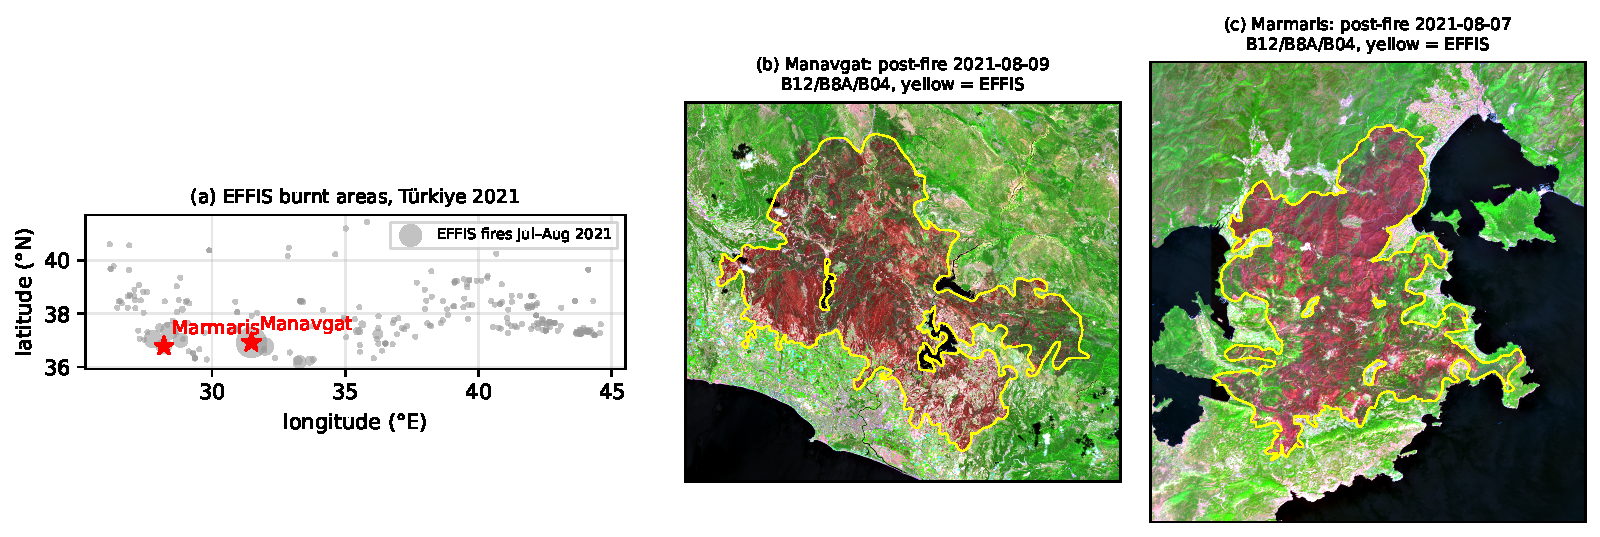
\includegraphics[width=0.9\textwidth]{study_area.pdf}
\caption{Study area. (a) EFFIS burnt areas in Türkiye, July--August 2021 (marker size $\propto$ area);
(b, c) post-fire Sentinel-2 false-colour composites (B12/B8A/B04) with the EFFIS perimeter.}\label{fig:study}
\end{figure*}

\textbf{Checks before testing.} BAM-CD with the official weights gives F1\,=\,\FoneBamcdOneFlogaSanity{} (v1) and
\FoneBamcdTwoFlogaSanity{} (v2) on our FLOGA test patches, close to the 88.48 reported in~\cite{sdraka2024floga};
the difference is plausible because our test patches use the v2 imagery and re-created unburnt patches. The
unburnt-land reflectance medians of FLOGA and the Turkish scenes differ by at most \HarmMaxAbsDiff{} in any band,
so the BOA-offset handling is consistent (Fig.~\ref{fig:harm}); the remaining differences, such as the darker SWIR
response of the Marmaris scenes, reflect land cover and atmosphere, i.e.\ genuine domain shift. HPO found LightGBM parameters with \HpLgbmNumLeaves{} leaves per tree and
learning rate \HpLgbmLearningRate{} (validation F1 \HpoValFoneLgbm{}, \HpoTrialsLgbm{} trials); the Random Forest
search was stopped by the 2\,h budget after \HpoTrialsRf{} trials (F1 \HpoValFoneRf{}). The LightGBM history
(Fig.~\ref{fig:hpo}) shows that all trials lie within one F1 point of the best one: the model is not sensitive to
its hyper-parameters, the number of leaves being the most important one. Early stopping on FLOGA validation stops
every LightGBM trial after fewer than 200 trees, a first sign that validation events differ from training events.

\begin{figure}[t]
\centering
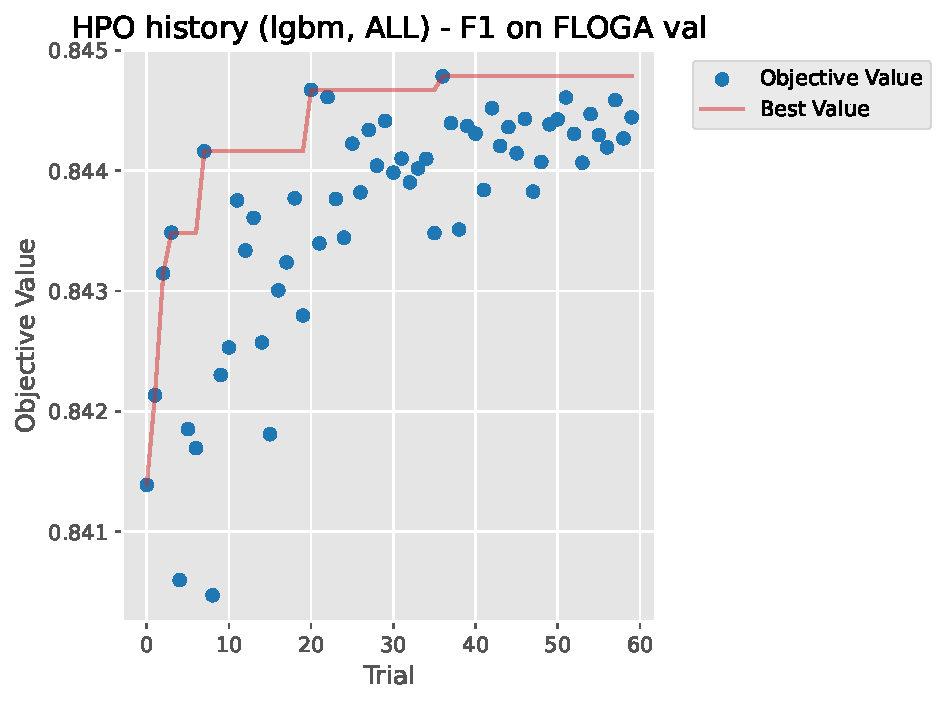
\includegraphics[width=0.85\columnwidth]{hpo_history_lgbm.pdf}
\caption{LightGBM hyper-parameter search: F1 on FLOGA validation per trial and best value so far.}\label{fig:hpo}
\end{figure}

\begin{figure}[t]
\centering
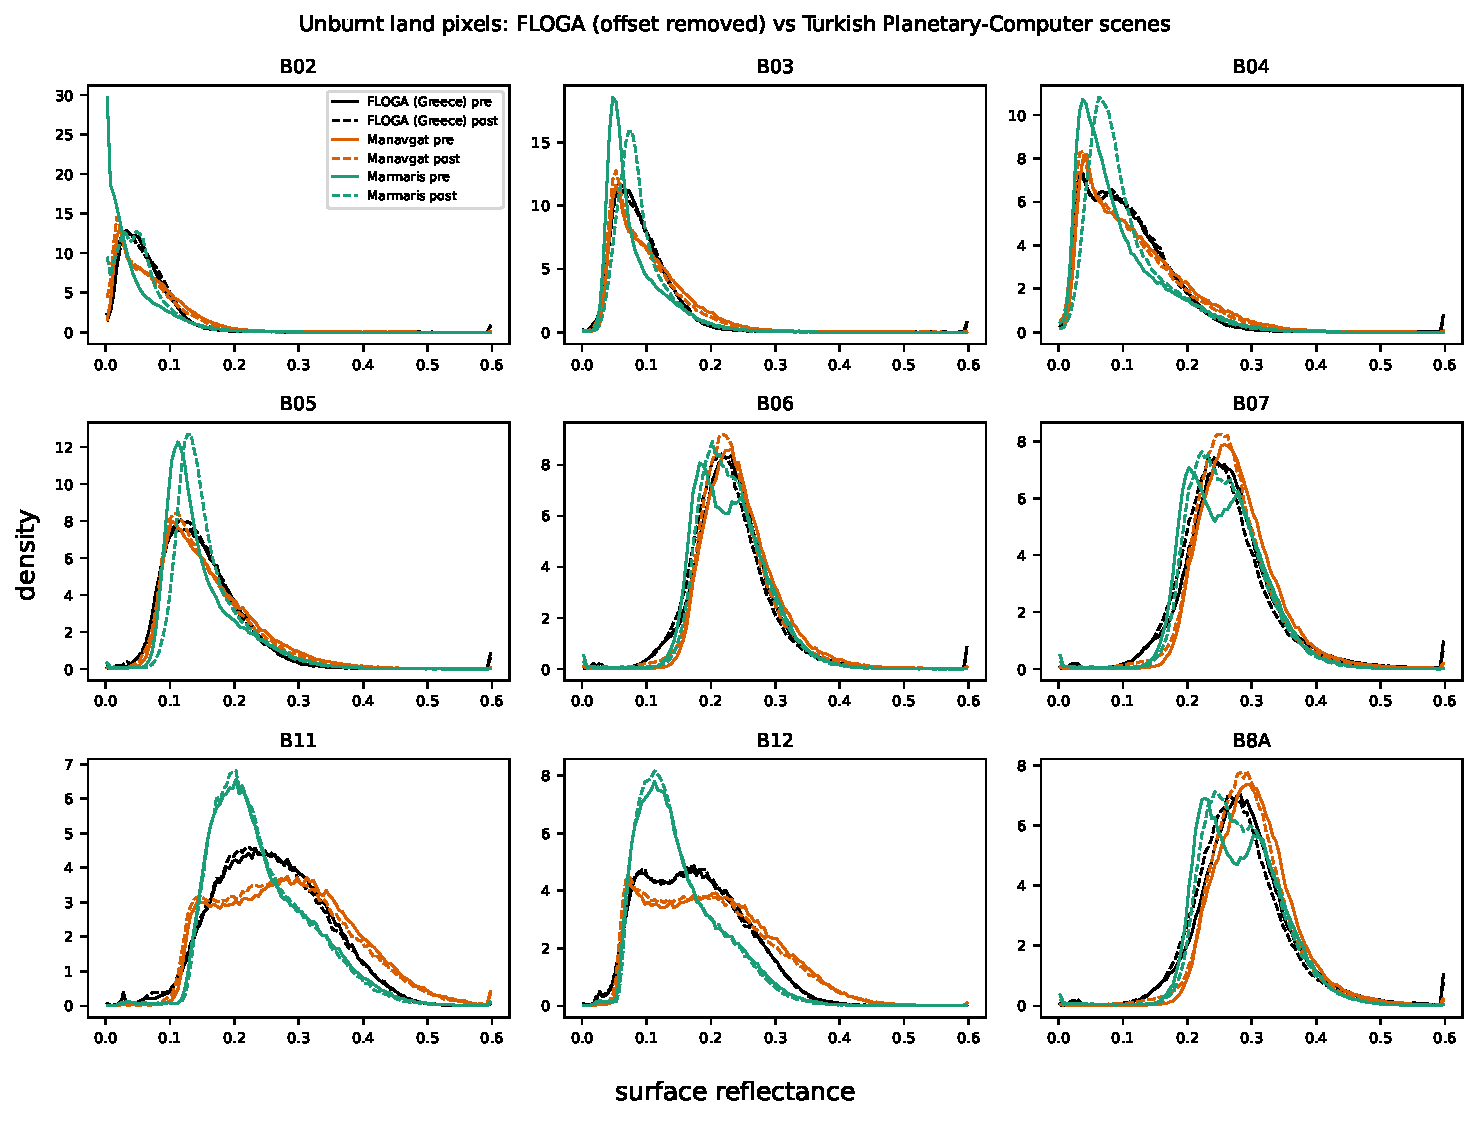
\includegraphics[width=\columnwidth]{band_harmonisation.pdf}
\caption{Reflectance distributions of unburnt land pixels in FLOGA (after removing the $+1000$ offset) and in the
Turkish pre- and post-fire scenes.}\label{fig:harm}
\end{figure}

\begin{table*}[t]
\centering
\caption{Burnt-class accuracy on the FLOGA test split and on the Turkish test events (EFFIS reference). Our models:
mean$\pm$std over 5 seeds. CI: 95\,\% spatial block bootstrap (1\,km blocks, 1000 resamples).}\label{tab:results}
\begin{tabular}{lcccccccc}
\toprule
 & FLOGA test & \multicolumn{2}{c}{Manavgat} & \multicolumn{2}{c}{Marmaris} & \multicolumn{2}{c}{T\"urkiye pooled} \\
Method & F1 & F1 & IoU & F1 & IoU & F1 & 95\% CI \\
\midrule
dNBR $>$ 0.27 (USGS) & 0.658 & 0.797 & 0.663 & 0.800 & 0.667 & 0.798 & [0.787, 0.809] \\
dNBR $>$ 0.10 (USGS) & 0.561 & 0.882 & 0.789 & \textbf{0.925} & 0.860 & 0.889 & [0.882, 0.897] \\
dNBR, FLOGA-val thr. & 0.661 & 0.822 & 0.698 & 0.831 & 0.711 & 0.824 & [0.813, 0.833] \\
BAM-CD v1 & 0.909 & 0.921 & 0.854 & 0.866 & 0.764 & 0.912 & [0.904, 0.921] \\
BAM-CD v2 & 0.913 & \textbf{0.931} & 0.872 & 0.893 & 0.806 & \textbf{0.925} & [0.917, 0.933] \\
LogReg (G2, ours) & 0.751 & 0.832 & 0.713 & 0.799 & 0.665 & 0.827 & [0.817, 0.837] \\
Random Forest (ours) & 0.865$\pm$0.001 & 0.886$\pm$0.000 & 0.795 & 0.857$\pm$0.002 & 0.750 & 0.881$\pm$0.001 & [0.873, 0.889] \\
LightGBM (ours) & 0.864$\pm$0.001 & 0.882$\pm$0.001 & 0.789 & 0.855$\pm$0.003 & 0.747 & 0.878$\pm$0.001 & [0.871, 0.887] \\
\bottomrule
\end{tabular}

\end{table*}

\textbf{Accuracy.} Table~\ref{tab:results} and Fig.~\ref{fig:metrics} summarise the results. On the Turkish
events pooled, LightGBM obtains F1\,=\,\FoneLgbmPooled{} (IoU \IoULgbmPooled) and the Random Forest
\FoneRfPooled; the seed-to-seed spread is at most a few thousandths. The paired bootstrap difference to BAM-CD v1 is
\DeltaLgbmBamcdOnePooled{} [\DeltaLgbmBamcdOnePooledLo, \DeltaLgbmBamcdOnePooledHi] pooled,
\DeltaLgbmBamcdOneManavgat{} [\DeltaLgbmBamcdOneManavgatLo, \DeltaLgbmBamcdOneManavgatHi] at Manavgat and
\DeltaLgbmBamcdOneMarmaris{} [\DeltaLgbmBamcdOneMarmarisLo, \DeltaLgbmBamcdOneMarmarisHi] at Marmaris, i.e.\ not
significant at Marmaris. BAM-CD v2 is better still (\FoneBamcdTwoPooled). Against the dNBR benchmark that is tuned,
like our models, on FLOGA only, LightGBM gains \DeltaLgbmDnbrFlogaPooled{}
[\DeltaLgbmDnbrFlogaPooledLo, \DeltaLgbmDnbrFlogaPooledHi] F1. The fixed USGS threshold dNBR\,$>$\,0.10 is
remarkably good on Türkiye (\FoneDnbrLowPooled, best of all methods at Marmaris) but poor on the FLOGA test split
(\FoneDnbrLowFloga), whereas our models score \FoneLgbmFloga{} there: the learned models are accurate in both
domains, the fixed threshold only in one. Our models are conservative: precision \PrecLgbmPooled{} versus recall
\RecLgbmPooled{} pooled, and the predicted area (\AreaLgbmPooled\,ha) is below the EFFIS area (\RefAreaPooled\,ha).

\begin{figure*}[t]
\centering
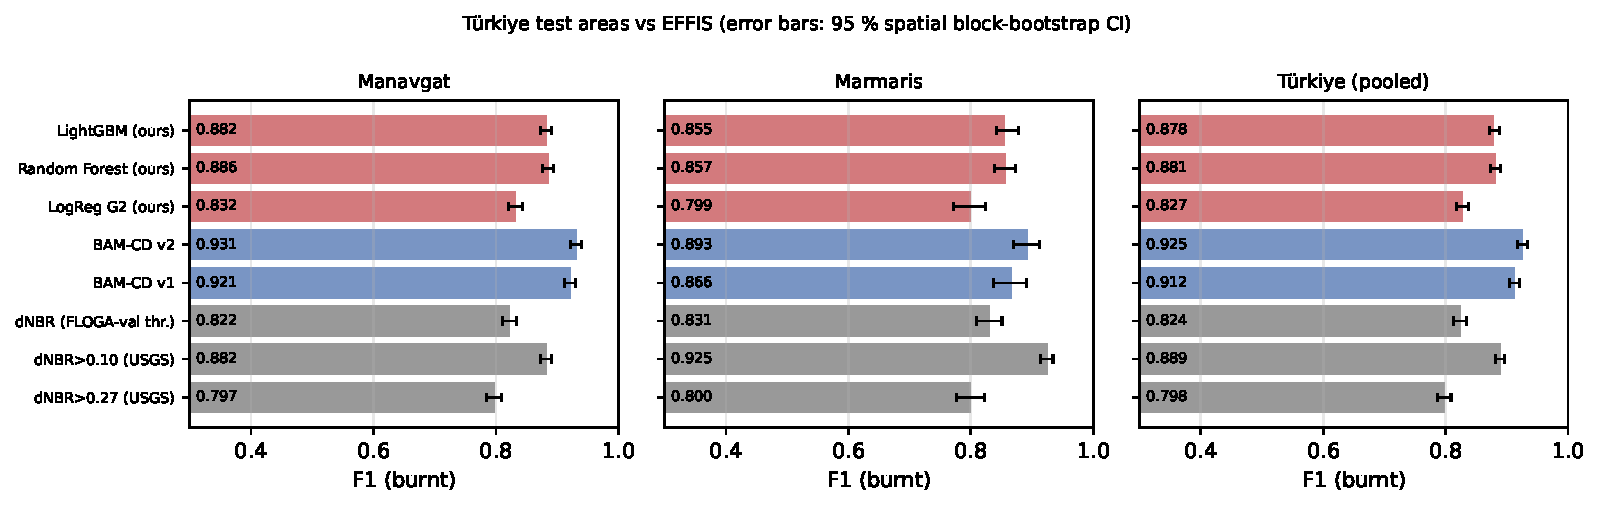
\includegraphics[width=\textwidth]{metrics_ci.pdf}
\caption{F1 on the Turkish events with 95\,\% block-bootstrap confidence intervals (seed 0 for our models).}\label{fig:metrics}
\end{figure*}

\textbf{Domain shift.} The F1 change from FLOGA test (in-domain) to Türkiye pooled (out-of-domain) is
\ShiftLgbm{} for LightGBM, \ShiftRf{} for the Random Forest and \ShiftBamcdOne{} for BAM-CD v1; no method lost
accuracy. The dNBR variants even gain more than 0.1 (\ShiftDnbrFloga{} for the FLOGA-tuned threshold), showing that
the two Turkish fires are easier targets than the average FLOGA test event: they are large, contiguous and
severely burnt, while FLOGA contains many small, partly burnt fires. The transfer is therefore successful, but
the absolute Turkish scores should not be read as typical for smaller Turkish fires.

\begin{figure*}[t]
\centering
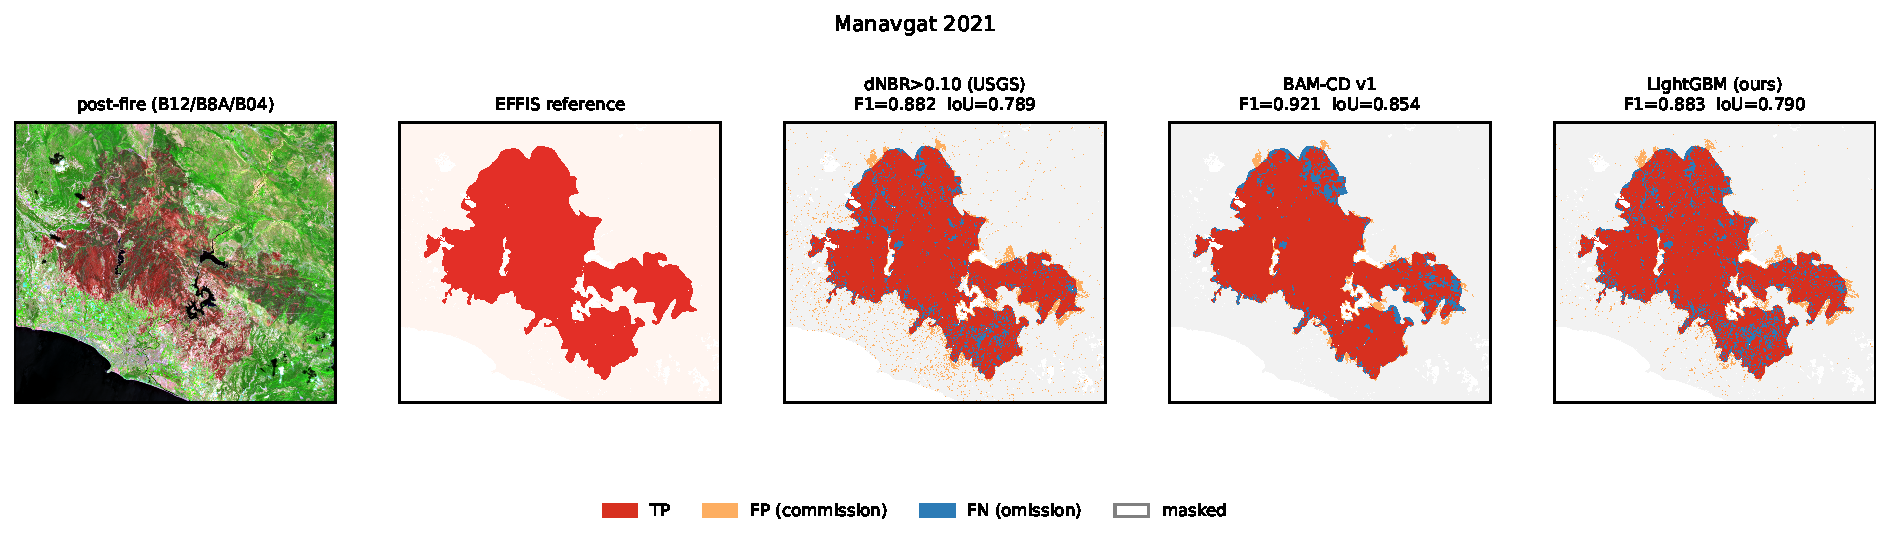
\includegraphics[width=\textwidth]{compare_Manavgat.pdf}\\[-2mm]
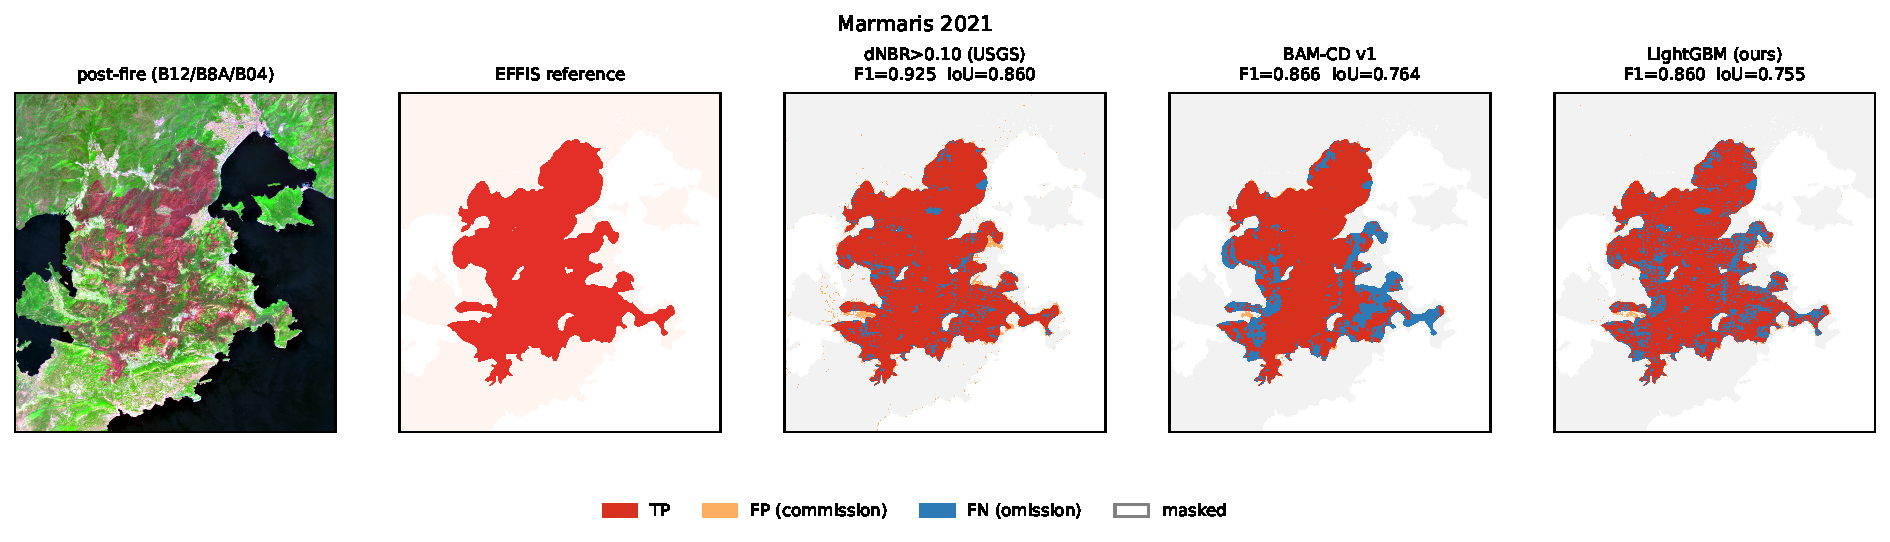
\includegraphics[width=\textwidth]{compare_Marmaris.pdf}
\caption{Agreement with EFFIS (red: true positive, orange: commission, blue: omission, white: masked) for dNBR,
BAM-CD v1 and LightGBM (seed 0). Most errors of all methods are omissions inside the EFFIS perimeter.}\label{fig:maps}
\end{figure*}

\textbf{Cost.} Table~\ref{tab:cost} and Fig.~\ref{fig:cost} compare cost on the same laptop. LightGBM predicts
1000\,km$^2$ in \CpuTimeLgbm\,s on the CPU, including feature computation, versus \CpuTimeBamcdOne\,s for BAM-CD
on the CPU and \GpuTimeBamcdOne\,s on the GPU; it trains in \TrainTimeLgbm\,s per seed and its model file is
\ModelMBLgbm\,MB, against \ModelMBBamcdOne\,MB of BAM-CD weights. The Random Forest is as accurate as LightGBM
but its fully grown trees make it \ModelMBRf\,MB large and about an order of magnitude slower (\CpuTimeRf\,s), so LightGBM is the better
lightweight choice. All methods run within a few gigabytes of RAM.

\begin{table}[t]
\centering
\caption{Cost on one laptop: parameters (tree nodes for forests), model size, training time per seed, inference
time per 1000\,km$^2$, peak RAM, and pooled Turkish F1 (F1 TR).}\label{tab:cost}
\resizebox{\columnwidth}{!}{\begin{tabular}{lrrrrrrr}
\toprule
Method & Params & MB & Train s & CPU s & GPU s & RAM MB & F1 TR \\
\midrule
dNBR $>$ 0.10 & 1 & 0.0 & 0 & 0.1 & -- & 445 & 0.889 \\
BAM-CD v1 & 83\,727\,022 & 319.4 & -- & 50.2 & 5.4 & 3786 & 0.912 \\
BAM-CD v2 & 126\,245\,998 & 481.6 & -- & 49.6 & 5.3 & 4497 & 0.925 \\
LogReg (G2, ours) & 7 & 0.0 & 0 & 0.9 & -- & 1337 & 0.827 \\
Random Forest & 14\,706\,552 & 1122.2 & 450 & 28.7 & -- & 3901 & 0.881 \\
LightGBM & 35\,834 & 1.9 & 9 & 2.9 & -- & 2765 & 0.878 \\
\bottomrule
\end{tabular}
}
\end{table}

\begin{figure}[t]
\centering
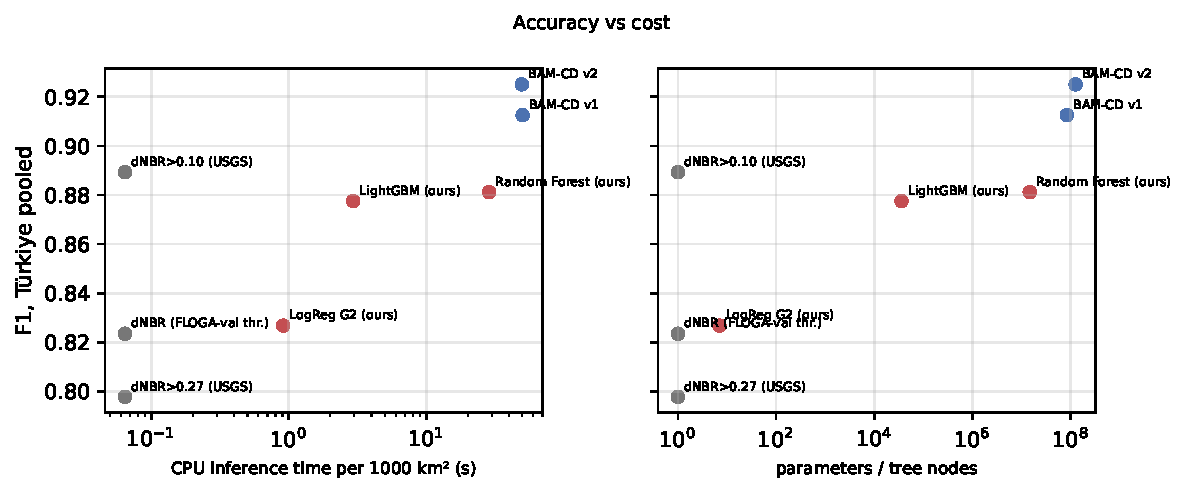
\includegraphics[width=\columnwidth]{cost_accuracy.pdf}
\caption{Accuracy versus cost (log axes).}\label{fig:cost}
\end{figure}

\begin{figure}[t]
\centering
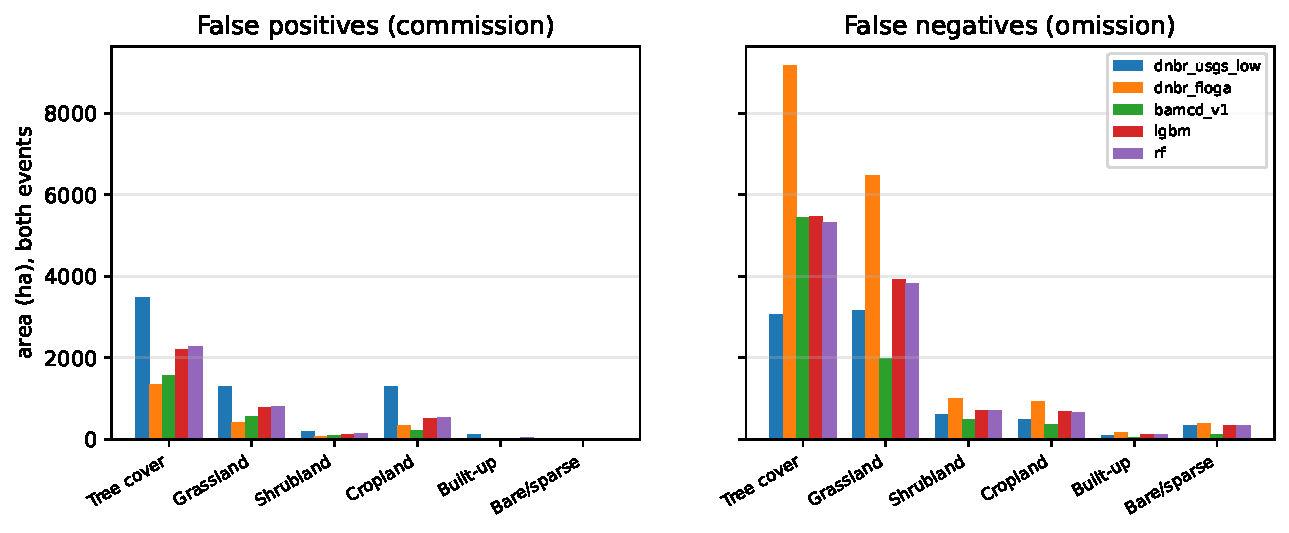
\includegraphics[width=\columnwidth]{errors_by_landcover.pdf}
\caption{Commission and omission area by ESA WorldCover 2021 class, both events.}\label{fig:errors}
\end{figure}

\begin{table}[!b]
\centering
\caption{Omission rate (\%) of EFFIS-burnt pixels per dNBR severity band (USGS classes), both events pooled, and
share of the reference in each band. Our models: seed 0.}\label{tab:severity}
\resizebox{\columnwidth}{!}{\begin{tabular}{lrrrrr}
\toprule
dNBR band & \% of ref. & dNBR, FLOGA-val thr. & BAM-CD v1 & Random Forest & LightGBM \\
\midrule
unburnt ($<$0.10) & 11.8 & 100.0 & 46.2 & 95.7 & 97.0 \\
low (0.10-0.27) & 19.9 & 78.9 & 24.5 & 20.8 & 23.1 \\
mod-low (0.27-0.44) & 23.3 & 0.0 & 8.5 & 2.7 & 2.7 \\
mod-high (0.44-0.66) & 20.7 & 0.0 & 2.0 & 0.6 & 0.3 \\
high ($\geq$0.66) & 24.3 & 0.0 & 0.4 & 2.1 & 1.7 \\
\bottomrule
\end{tabular}
}
\end{table}

\textbf{Ablation.} The models of Table~\ref{tab:ablation} retrain LightGBM (same hyper-parameters,
5 seeds) on nested feature groups. dNBR alone (G1) reaches only \AblGOneVal{} on FLOGA validation; the six
differenced indices (G2) raise it to \AblGTwoVal{}, which is most of the gain. Post-fire bands (G2+G3,
\AblGTwoThreeVal) and pre-fire bands and single-date indices (ALL, \AblAllVal) add little on FLOGA. On Türkiye the
picture differs by event: ALL is best at Manavgat (\FoneLgbmManavgat), while G2+G3 is better at Marmaris
(\FoneAblGTwoThreeMarmaris{} vs \FoneLgbmMarmaris). Pre-fire reflectance carries site-specific information (the
Marmaris pre-fire scene is darker in the SWIR bands than FLOGA), which can hurt transfer. Following our protocol, the
main model was fixed on FLOGA validation (ALL) and not changed after seeing this test result.

\begin{table}[t]
\centering
\caption{Feature ablation (LightGBM, F1, mean$\pm$std over 5 seeds). G1: dNBR; G2: six differenced indices;
G3: post-fire bands; ALL: G2+G3+pre-fire bands+single-date indices.}\label{tab:ablation}
\resizebox{\columnwidth}{!}{\begin{tabular}{lrcccc}
\toprule
Features & \# & FLOGA val & FLOGA test & Manavgat & Marmaris \\
\midrule
G1 & 1 & 0.678$\pm$0.000 & 0.661$\pm$0.000 & 0.819$\pm$0.004 & 0.827$\pm$0.005 \\
G2 & 6 & 0.839$\pm$0.000 & 0.867$\pm$0.001 & 0.862$\pm$0.001 & 0.831$\pm$0.003 \\
G2+G3 & 15 & 0.841$\pm$0.000 & 0.861$\pm$0.001 & 0.874$\pm$0.001 & 0.875$\pm$0.002 \\
ALL & 36 & 0.844$\pm$0.000 & 0.864$\pm$0.001 & 0.882$\pm$0.001 & 0.855$\pm$0.003 \\
\bottomrule
\end{tabular}
}
\end{table}

\textbf{Error analysis.} Fig.~\ref{fig:maps} and Fig.~\ref{fig:errors} break the errors down by ESA WorldCover
class. For all methods, omission errors are larger than commission errors and concentrate in tree cover and
grassland inside the EFFIS perimeter. Part of this is unburnt or lightly burnt vegetation that EFFIS includes in
its generalised perimeter (unburnt islands), so it is not necessarily a model error. Compared with BAM-CD, our
pixel models miss more burnt grassland, cropland and bare or sparse land, where the spectral change is weak and
BAM-CD can use the spatial context of neighbouring pixels. Commission of our models is small and mostly at the
perimeter edges; dNBR\,$>$\,0.10 produces the most scattered false alarms on cropland outside the fires.

Table~\ref{tab:severity} groups the EFFIS-burnt pixels by their own dNBR. \SevShareUnchanged\,\% of them show
almost no spectral change (dNBR\,$<$\,0.10). A pixel classifier can hardly label such pixels as burnt: LightGBM
misses \SevOmitUnchangedLgbm\,\% of them and the Random Forest \SevOmitUnchangedRf\,\%. BAM-CD misses only
\SevOmitUnchangedBamcdOne\,\%, because its convolutional decoder fills small unchanged patches enclosed by burnt
land, as EFFIS's generalised perimeter does. In the moderate and high severity bands our models omit fewer
burnt pixels than BAM-CD. Hence BAM-CD's higher recall on Türkiye comes mainly from pixels whose ``burnt'' label is
a property of the perimeter rather than of the spectral signal.



\section{Discussion}\label{sec:discussion}
\textbf{Where and why.} The lightweight model closes most of the gap between dNBR and BAM-CD at a small fraction
of BAM-CD's cost, and it is the only method that is good on both FLOGA and Türkiye without per-site threshold
tuning. Its remaining gap to BAM-CD comes from pixels with weak spectral change, where spatial context matters;
adding simple neighbourhood features (e.g.\ local means of dNBR) is a natural next step.

\textbf{Operational use.} For OGM and AFAD the practical question is which tool to run after the next fire. On a
standard office CPU LightGBM maps 1000\,km$^2$ in seconds, needs no GPU and fits in an e-mail attachment, so it
can be run for every fire of a season; the map is conservative (high precision), which suits damage statistics
that must not be inflated. BAM-CD gives the most complete perimeters and is preferable when a GPU is available
and a single large fire must be mapped as completely as possible. A fixed dNBR threshold is the cheapest option,
but our results show that the right threshold differs between regions (0.10 fits Türkiye, the FLOGA-tuned
\DnbrFlogaThr{} fits Greece), which a learned model avoids.

\textbf{Why no domain-shift loss?} One might expect a model trained in Greece to degrade in Türkiye. Both countries
share Mediterranean climate, vegetation types (pine forest and maquis) and the same sensor and processing
chain, and our harmonisation removed the only systematic radiometric difference (the BOA offset). The ablation
nevertheless shows a residual site effect: pre-fire bands help at Manavgat but hurt at Marmaris, so features that
describe the \emph{change} transfer better than features that describe the \emph{site}.

\textbf{Limitations.} (i) The reference is EFFIS, which is itself mapped from Sentinel-2 by analysts with
spectral-index tools; it is independent of our models but not of the sensor, and its generalised perimeters
include unburnt islands. This may also explain why dNBR\,$>$\,0.10 matches it so well. An independent check with
photo-interpreted points is prepared (\texttt{labeling/}) but not yet labelled. (ii) Only two events from one
season were tested, both large and severe; smaller or low-severity fires are likely harder. (iii) FLOGA v1
imagery could not be downloaded by code, so we used the reprocessed v2 imagery and re-created the unburnt patch
selection; BAM-CD v1 was trained on v1 imagery, although its FLOGA test score is close to the published one.
(iv) The bootstrap CIs use one seed per method; the seed-to-seed spread is reported separately and is much
smaller than the CIs. (v) The Random Forest search used \HpoTrialsRf{} of 60 trials within the 2\,h budget.

\section{Conclusion and Future Work}\label{sec:conclusion}
A LightGBM classifier trained only on Greek FLOGA data maps the 2021 Manavgat and Marmaris burnt areas with
F1\,=\,\FoneLgbmPooled{} against EFFIS ($\Delta$F1\,=\,\DeltaLgbmBamcdOnePooled{} relative to the BAM-CD deep
network) and clearly above
a FLOGA-tuned dNBR, while running \SpeedupCpuLgbmBamcd$\times$ faster on a CPU with a \ModelMBLgbm\,MB model. Transfer
from Greece to Türkiye did not reduce the accuracy of any method. Future work: independent check labels,
more and smaller Turkish fires (e.g.\ the other 2021 EFFIS events), neighbourhood features, and a light
fine-tuning step with a few Turkish labels.

\section*{Code and Data Availability}
Code, configuration, small models, all tables and figures: \url{https://github.com/html37/ehb466-burnt-area-tr},
release \texttt{v1.0}. \texttt{run\_all.py} regenerates every number of this paper, and a Colab notebook runs the
demo end to end. Data: Sentinel-2 L2A via Microsoft Planetary Computer (Copernicus licence), FLOGA (CC BY 4.0),
EFFIS (\textcopyright{} European Union), ESA WorldCover (CC BY 4.0), BAM-CD code (MIT) and weights from the FLOGA
repository.

\section*{Author Contributions and Use of AI}
\textbf{[TODO: confirm roles]} H.~Temel and E.~Akkoca: roles to be stated with CRediT terms by the authors.
Claude Code (Anthropic) was used for code generation, experiment orchestration and drafting of the text; the
authors reviewed all code, results and text and are responsible for the content.


\bibliographystyle{IEEEtran}
\bibliography{refs}

\end{document}
